\chapter{Statistical analysis and results}
\label{chap:statandresults}

\ifNewAnalysis
The signal and background models described in \Chapter~\ref{chap:model} are used to perform the statistical interpretation of the \thisanalysislumi\ifb of data. The result is an independent observation of the Higgs boson in the diphoton decay channel and measurements of some of its properties. %The objective is to twofold:
\else
The signal and background models described in \Chapter~\ref{chap:model} are used to perform the statistical interpretation of \thisanalysislumi\ifb of \RunII data collected at $\sqrt{s}=13\TeV$ by \CMS in 2016. The author was responsible for the signal and background modelling, systematics handling and statistical interpretation in the official \CMS preliminary result~\cite{CMS-PAS-HIG-16-020} produced with the same dataset. The results presented in this section differ from those presented in~\cite{CMS-PAS-HIG-16-020} insofar as they use improvements to the signal modelling techniques developed by the author. Namely the \DCBpG functional form was used instead of a sum of Gaussians, and interpolation using \SSF was used instead of linear interpolation. The results from this thesis and~\cite{CMS-PAS-HIG-16-020} are almost identical, as expected, and are compared at various points throughout this chapter.

Due to the scaling of the \SM Higgs boson and background \crosssection\s moving from 7 or 8\TeV to 13\TeV, the dataset used in this thesis has roughly the same statistical sensitivity as the full \RunI dataset, which had an integrated luminosity of $24.8\ifb$. The final analysis of the \RunI dataset~\cite{LegacyHgg} led to an independent observation of the Higgs boson in the diphoton decay channel. The objective of the work presented in this thesis is therefore to make a confirmation of the observation (or ``rediscovery'') of the Higgs boson in the diphoton decay channel, and measurements of some of its properties.
\fi

The statistical analysis proceeds in several stages. The first step is to determine the best signal-plus-background fit of the models to the data. The floating parameters of the signal and background models are varied simultaneously in each analysis category to obtain the closest overall agreement with the observed invariant mass distributions. This procedure is described in \Sec~\ref{sec:statandresults:bestfit}, and leads to a Higgs boson signal being measured in the data. The next step is to quantify the significance of this signal and formally reject the hypothesis that there is no Higgs boson. The procedure for hypothesis testing and calculation of the significance is detailed in \Sec~\ref{sec:statandresults:significance}. Having established the existence of a \SM-like Higgs boson which decays to photons, the final step is to make measurements of some of its properties, in particular those which relate to the rate at which it is produced or interacts with other \SM particles. These measurements are described in \Sec~\ref{sec:statandresults:sigstrength} and \Sec~\ref{sec:statandresults:kappas}. 
 
As with all Higgs boson analyses performed within the \CMS collaboration, the statistical interpretation uses the frequentist approach. The corresponding statistical tools and techniques are briefly explained as they are needed throughout this chapter.

\section{Best fit of models to the data}
\label{sec:statandresults:bestfit}

The observed \mgg distributions obtained from the data (labelled $ \mgg^{obs}$ hereafter) are parametrised with models consisting of signal and background components. The tool which is used determine the model parameters and to assess the agreement with the data in a category $C$ is called the \emph{likelihood function},
\begin{equation}
\label{eq:statandresults:likelihood_function}
\mathcal{L}_C(\mu, \mH; \mathbf{n} | \mgg^{obs,C} ) = \mu \cdot f^C_S(\mgg^{obs,C} |\mH ; \mathbf{n}_S) + f^C_B(\mgg^{obs,C} | \mathbf{n}_B ). 
\end{equation}
In the definition above:
\begin{itemize}
\item $\mu = \sigma^{H} / \sigma^{H}_{SM}$ is a \POI called the signal strength, where in this context $\sigma^H$ is the observed Higgs boson cross section, and $\sigma^H_{SM}$ is the \SM Higgs boson \crosssection. The mass of the Higgs boson \mH is a second \POI. The likelihood function can in fact be generalised for an arbitrary number of \POI\s (as in \Sec\s~\ref{sec:statandresults:sigstrength} and~\ref{sec:statandresults:kappas}); 
\item $\mathbf{n}$ is a set of floating nuisance parameters, composed of those which affect the signal model and those which affect the background model, labelled $\mathbf{n}_S$ and $\mathbf{n}_B$ respectively;
\item $\mgg^{obs,C}$ is the invariant mass distribution for a particular category $C$;
\item $f^C_S$ and $f^C_B$ represent the probability distribution functions of the signal and background components of the model in category $C$, normalised to the expected number of signal and background events in that category respectively. Some of the nuisances parameters can modify the normalisation of $f^C_S$ and $f^C_B$. 
\end{itemize}

The construction of the signal component of the model in each category, $f^C_S$, was described in \Sec~\ref{model:sec:signal_model}, and is comprised of the individual models for each Higgs boson production process, each normalised to their respective expected number of events:
\begin{equation}
\label{eq:statandresults:f_s_breakdown}
\begin{split}
 f^C_S(\mgg^{obs,C} |\mH ; \mathbf{n}_S) ={} & f^C_{S,{\text{ggH}}}(\mgg^{obs,C} |\mH ; \mathbf{n}_S)  + f^C_{S,{\text{VBF}}}(\mgg^{obs,C} |\mH ; \mathbf{n}_S)\\
  & + f^C_{S,{\text{VH}}}(\mgg^{obs,C} |\mH ; \mathbf{n}_S)+ f^C_{S,{\text{ttH}}}(\mgg^{obs,C} |\mH ; \mathbf{n}_S).\\
\end{split}
\end{equation}

When performing the signal-plus-background fit to the data, the values of the individual parameters of the signal model functional form are fixed. Specifically, since the \SSF method was used, this refers to the coefficients of the seventeen polynomial functions which describe the dependence on \mH of the \DCBpG parameters for both the \RV and \WV scenarios and their mixing fraction. The parameters which are allowed to vary are the nuisance parameters $\mathbf{n}_S$ introduced into the signal modelling to account for systematic uncertainties (see \Sec~\ref{model:sec:systematics}), as well as the \POI\s $\mu$ and \mH. The signal strength $\mu$ uniformly scales all the signal models for each process and for each category. This means that the contribution to the overall signal model from each process remains in proportion to what is predicted by the \SM, but the normalisation of the overall signal model can be varied.

The handling of the background component of the model $f^C_B$, for a given category, was described in \Sec~\ref{model:sec:background_model}. The nuisance parameters $\mathbf{n}_B$ affecting the background model are composed of:
\begin{itemize}
\item the discrete nuisance parameter in each category which corresponds to the choice of background function, as prescribed by the discrete profiling method (see \Sec~\ref{model:sec:background_model_envelope}); 
\item the individual parameters of all the candidate functions, in all categories, which are allowed to float in the fit.
\end{itemize}

The overall likelihood function $\mathcal{L}$ for the simultaneous fit of all categories at once is obtained by taking the product of the likelihood functions $\mathcal{L}_C$ in each analysis category, taking care to correlate the corresponding nuisance parameters in each one:
\begin{equation}
\label{eq:statandresults:likelihood_function_product}
\mathcal{L}(\mu, \mH; \mathbf{n} | \mgg^{obs} ) = \prod_{C} \mathcal{L}_C(\mu, \mH; \mathbf{n} | \mgg^{obs,C} ).
\end{equation}

%The fit is obtained by minimising twice the negative log-likelihood ($ -2 \ln \mathcal{L}(\mu, \mH ; \mathbf{n}| \mgg^{obs}$) or \NLL). 
The fit is obtained by minimising twice the negative log-likelihood (\NLL). 
The best-fit values of the \POI\s and nuisance parameters are denoted as $\hat{\mu}$, $\hat{\mH}$ and $\hat{\mathbf{n}}$, such that:
\begin{equation}
%(\hat{\mu}, \hat{\mH} , \hat{\mathbf{n}}) = 
\{ (\mu, \mH, \mathbf{n}) : -2 \ln \mathcal{L}(\hat{\mu}, \hat{\mH} ;\hat{\mathbf{n}}| \mgg^{obs}) = \min _{\mu,\mH , \mathbf{n}}(-2 \ln \mathcal{L}(\mu, \mH; \mathbf{n}| \mgg^{obs})) \},
\end{equation}
where $\displaystyle\min_{ \mu, \mH ,\mathbf{n}}$ represents the global minimum evaluated over all allowed values of $\mu$, \mH and $\mathbf{n}$, taking into account their constraints. The parameters in this analysis are constrainted in one of three possible ways: for the systematic uncertainties described by shape nuisances, a Gaussian constraint is applied ; for the systematic uncertainties described by yield or migration nuisances, a log-normal constrain is applied ; for all other nuisances, the constraint is flat. 

 In general, the \NLL cannot be minimized analytically. Instead, this task is handled numerically with the \Minuit minimizer~\cite{minuit}, as part of the \RooFit software package~\cite{RooFit}. 
The resulting parametrisations of the observed data are shown for each analysis category separately in \Fig\s~\ref{fig:statandresults:s_b_fits} and~\ref{fig:statandresults:s_b_fits_bis}. The combined parametrisation and data resulting from a direct sum of each category is shown in \Fig~\ref{fig:statandresults:s_b_fits_direct_sum}, while the sum weighted by the $S/(S+B)$ in $\pm \effSigma$ around the best-fit $\mH$ in each category is shown in \Fig~\ref{fig:statandresults:s_b_fits_s_sb_sum}. 

\begin{figure}[p]
\centering
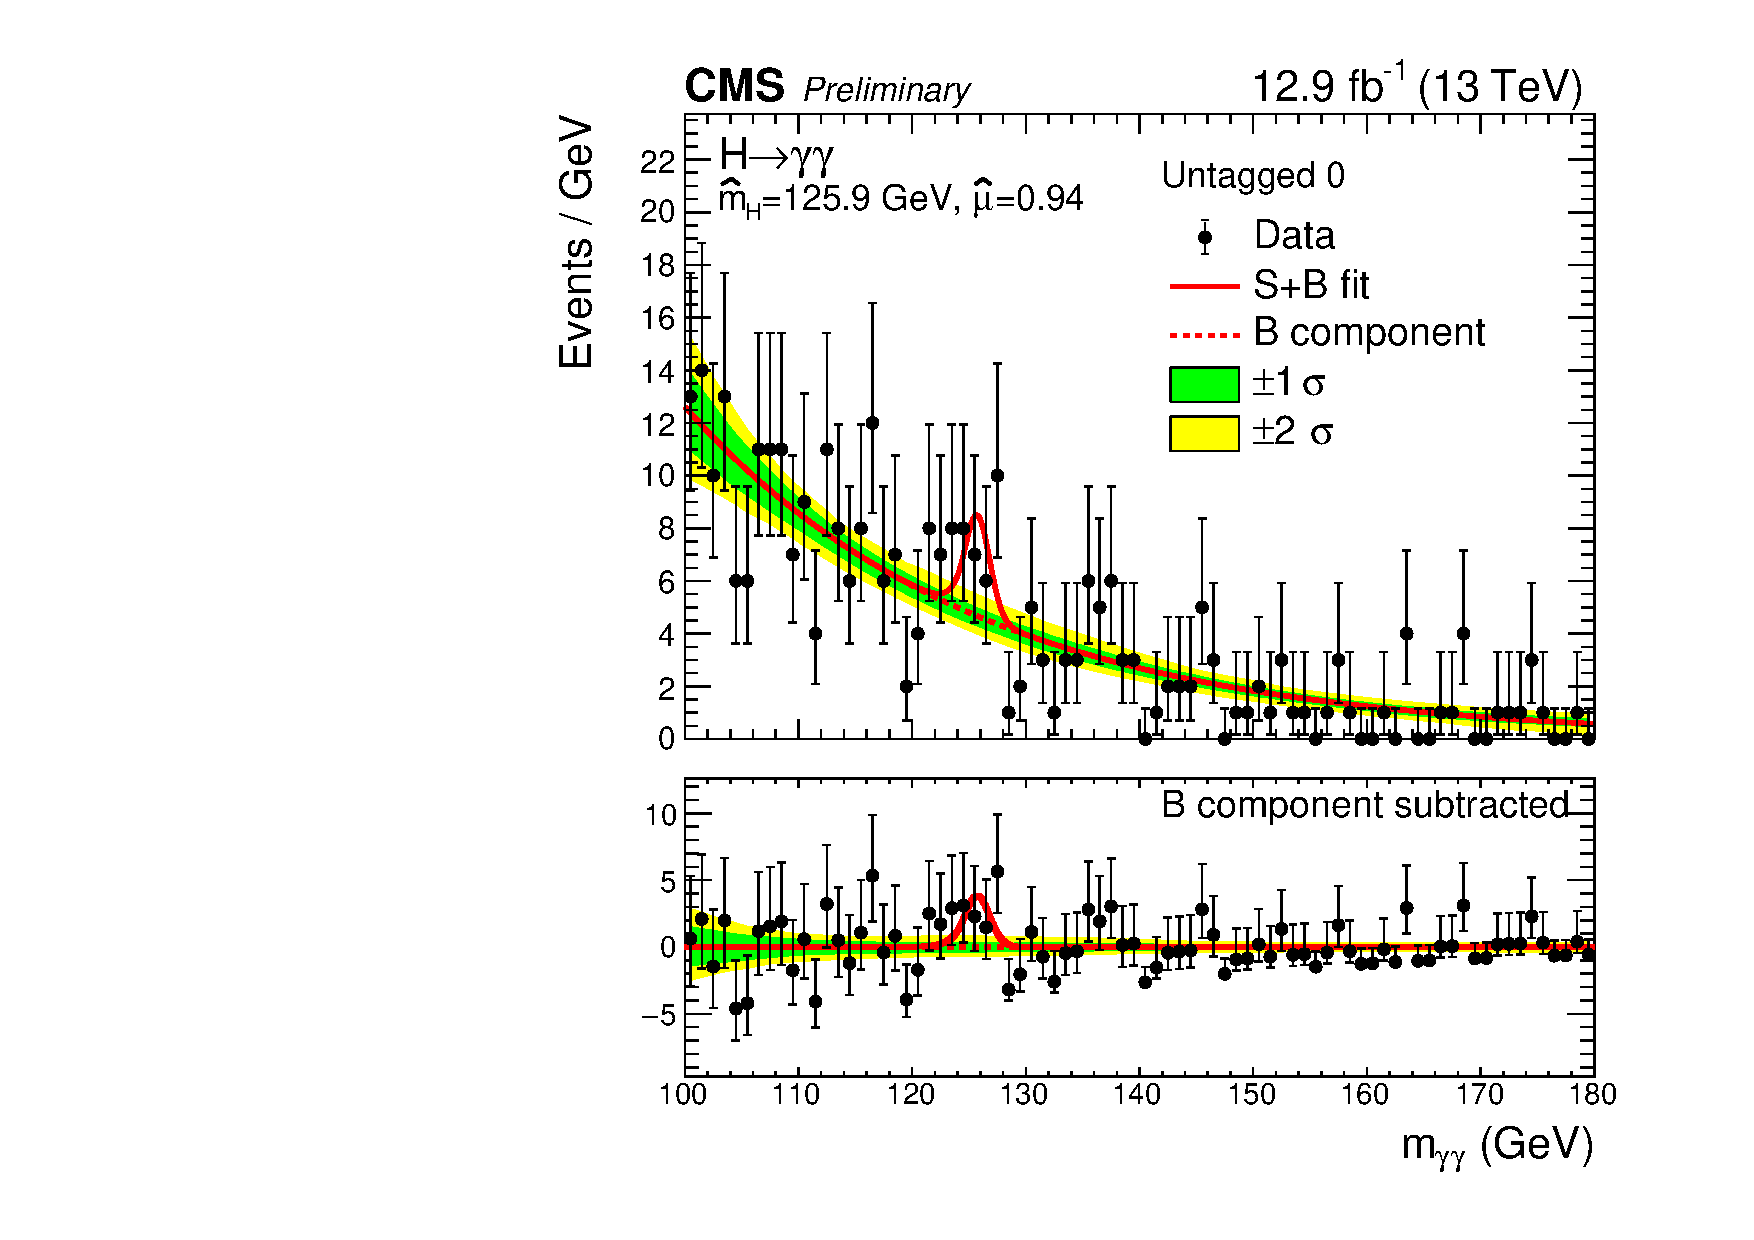
\includegraphics[width=0.49\textwidth]{statandresultsFigures/\whichFig/S_SB_ProfileMH_UntaggedTag_0_13TeV.pdf} 
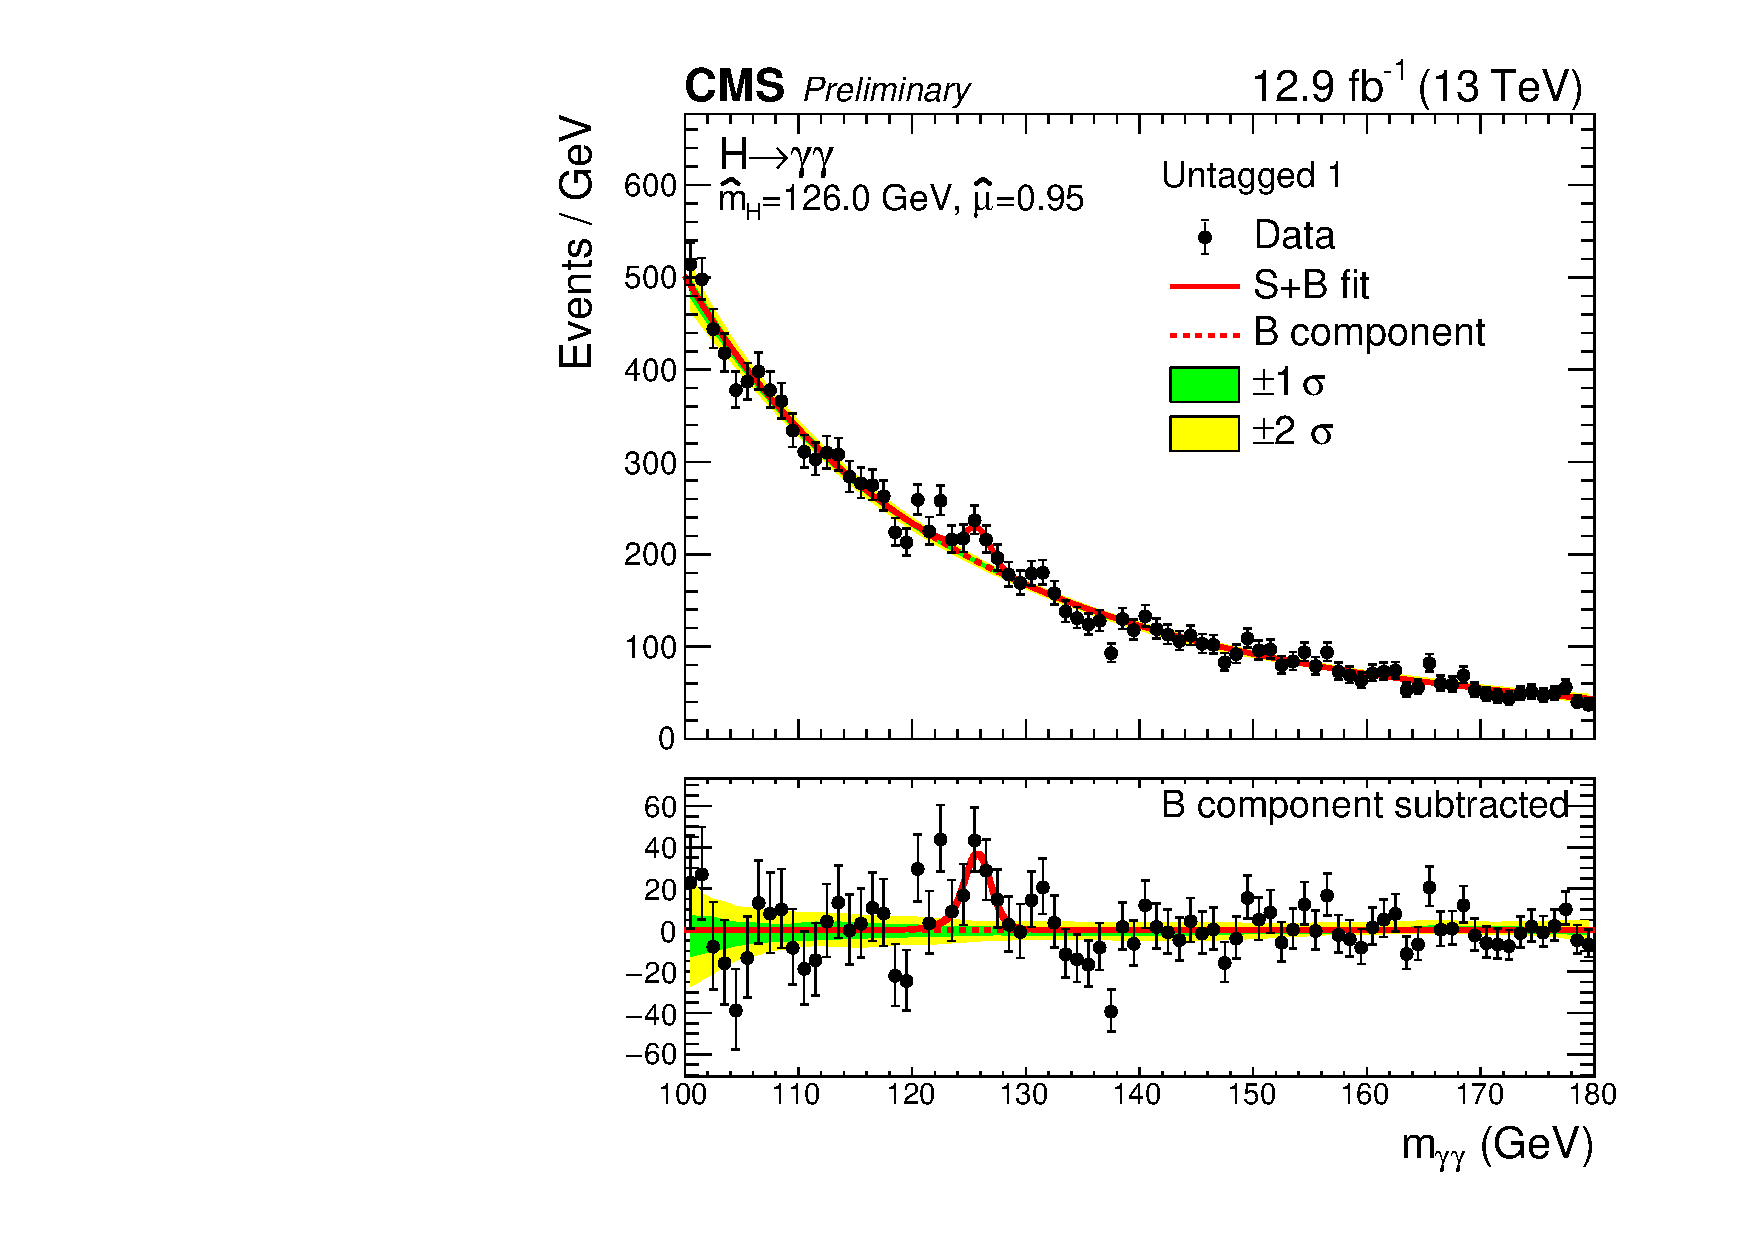
\includegraphics[width=0.49\textwidth]{statandresultsFigures/\whichFig/S_SB_ProfileMH_UntaggedTag_1_13TeV.pdf}\\ 
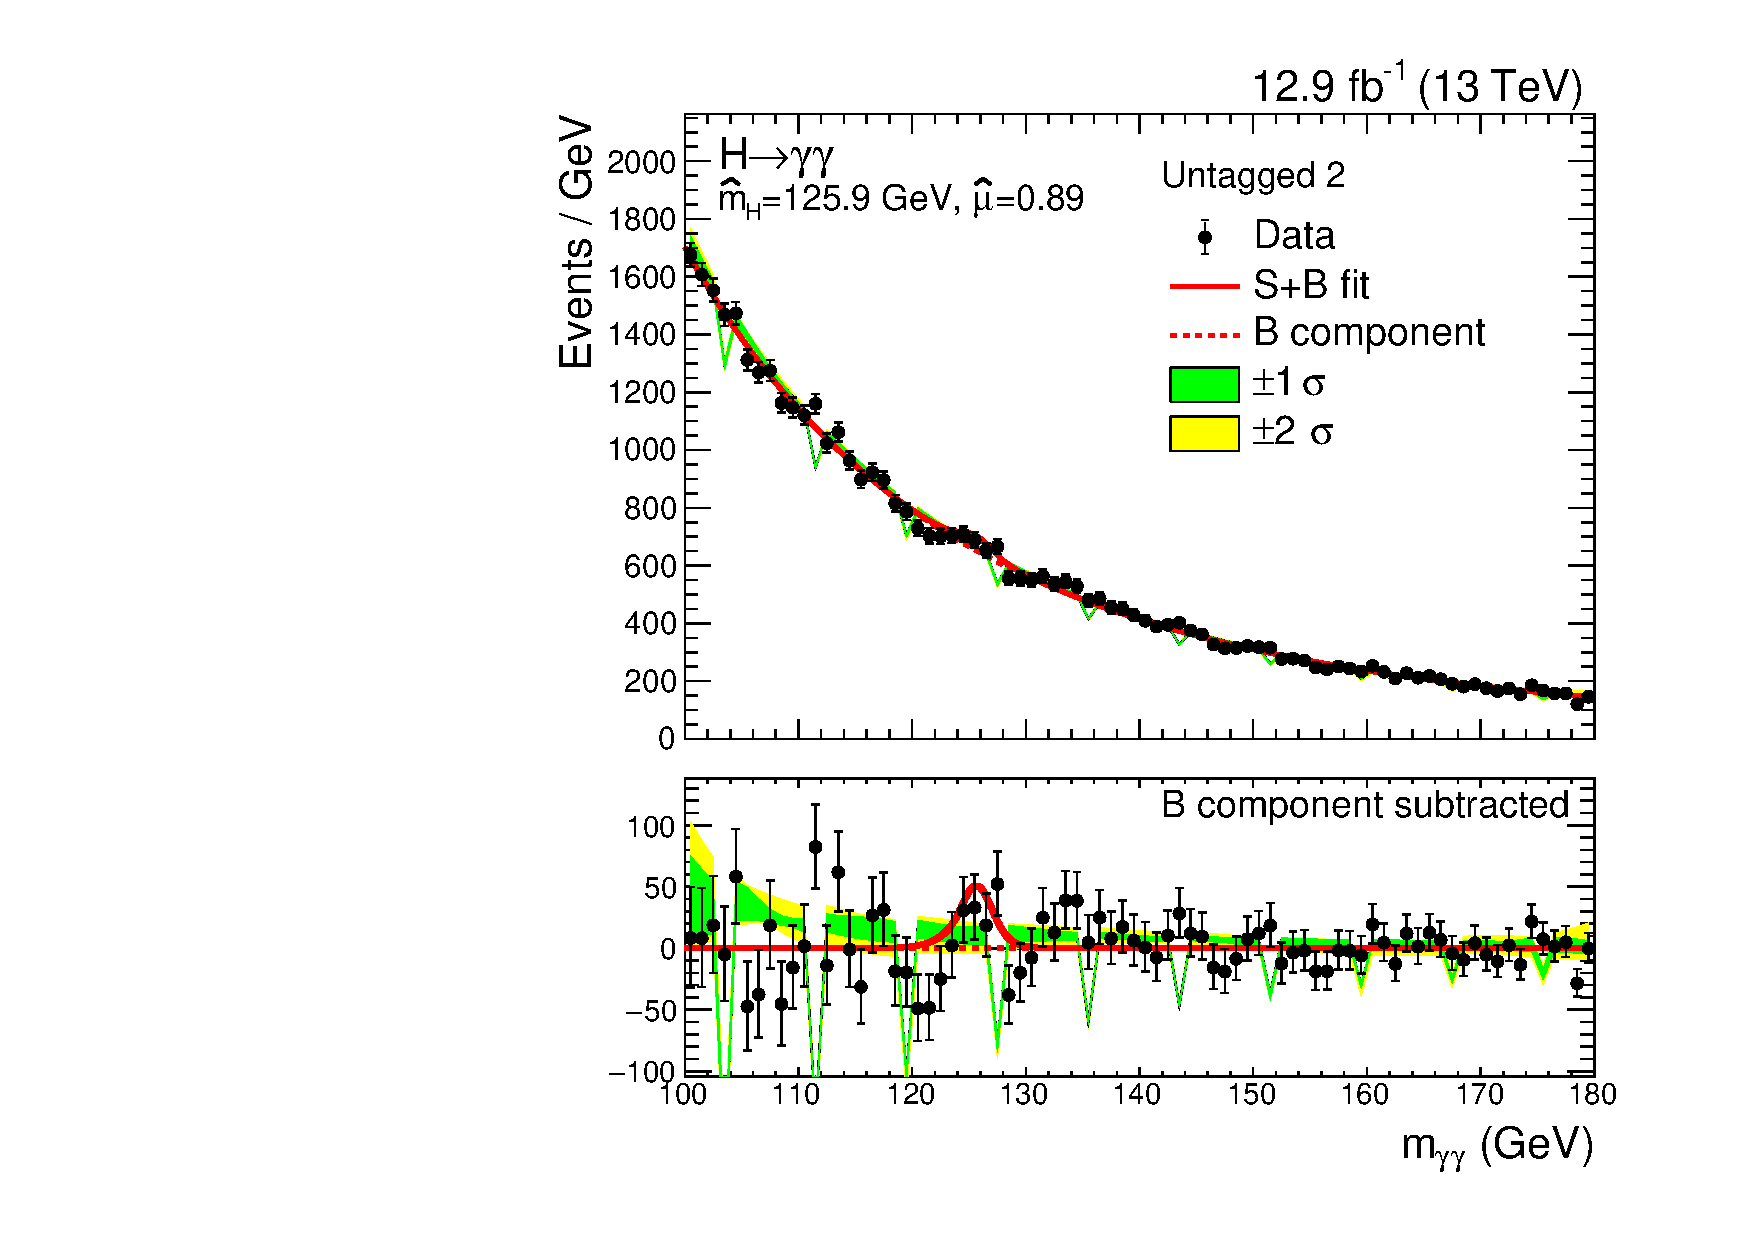
\includegraphics[width=0.49\textwidth]{statandresultsFigures/\whichFig/S_SB_ProfileMH_UntaggedTag_2_13TeV.pdf} 
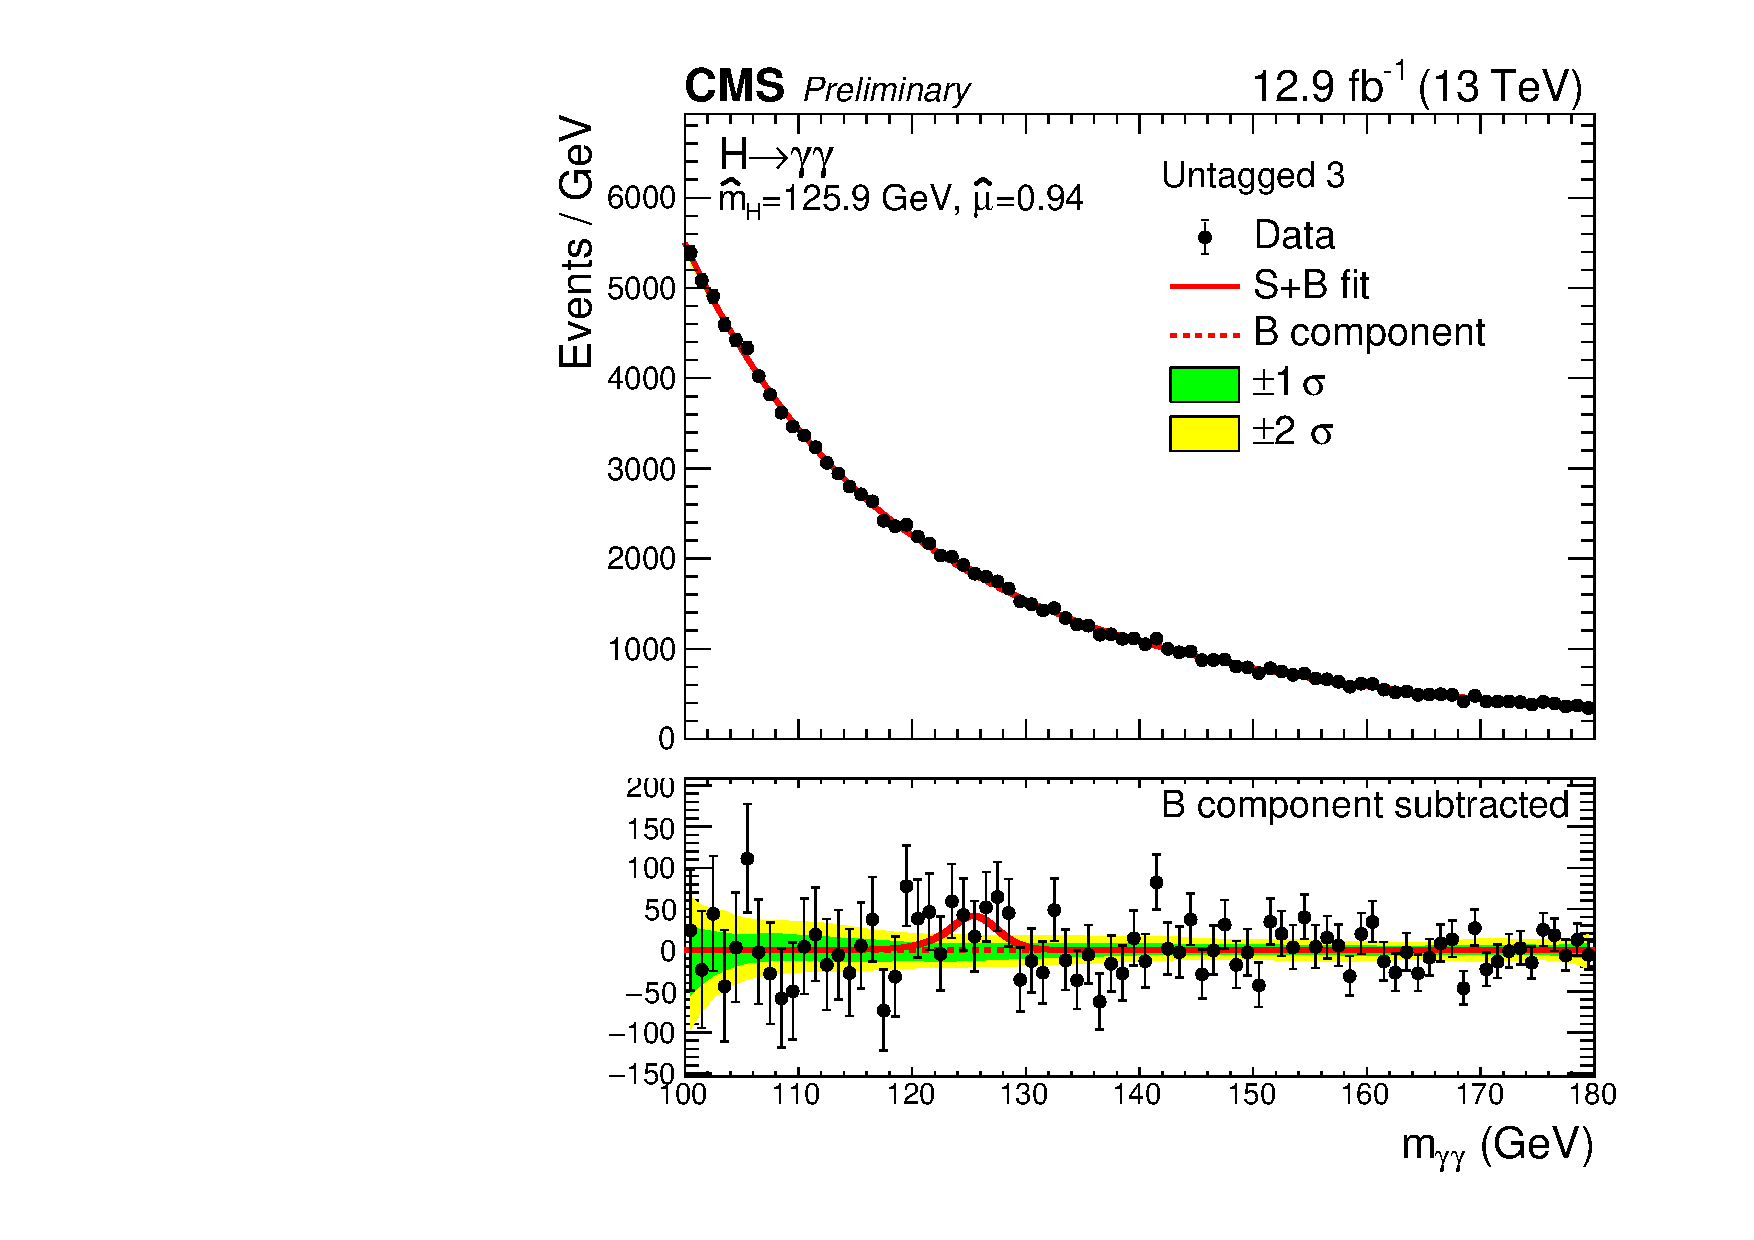
\includegraphics[width=0.49\textwidth]{statandresultsFigures/\whichFig/S_SB_ProfileMH_UntaggedTag_3_13TeV.pdf} \\
\caption{The signal-plus-background fit (solid red line) of the observed \mgg distribution in data (black points) for the \Untagged analysis categories. The background-only fit is shown as a dashed red line, while the green and yellow bands denote the $1\sigma$ and $2\sigma$ uncertainties on the background shape respectively.}

\label{fig:statandresults:s_b_fits}
\end{figure}

\begin{figure}[p]
\centering
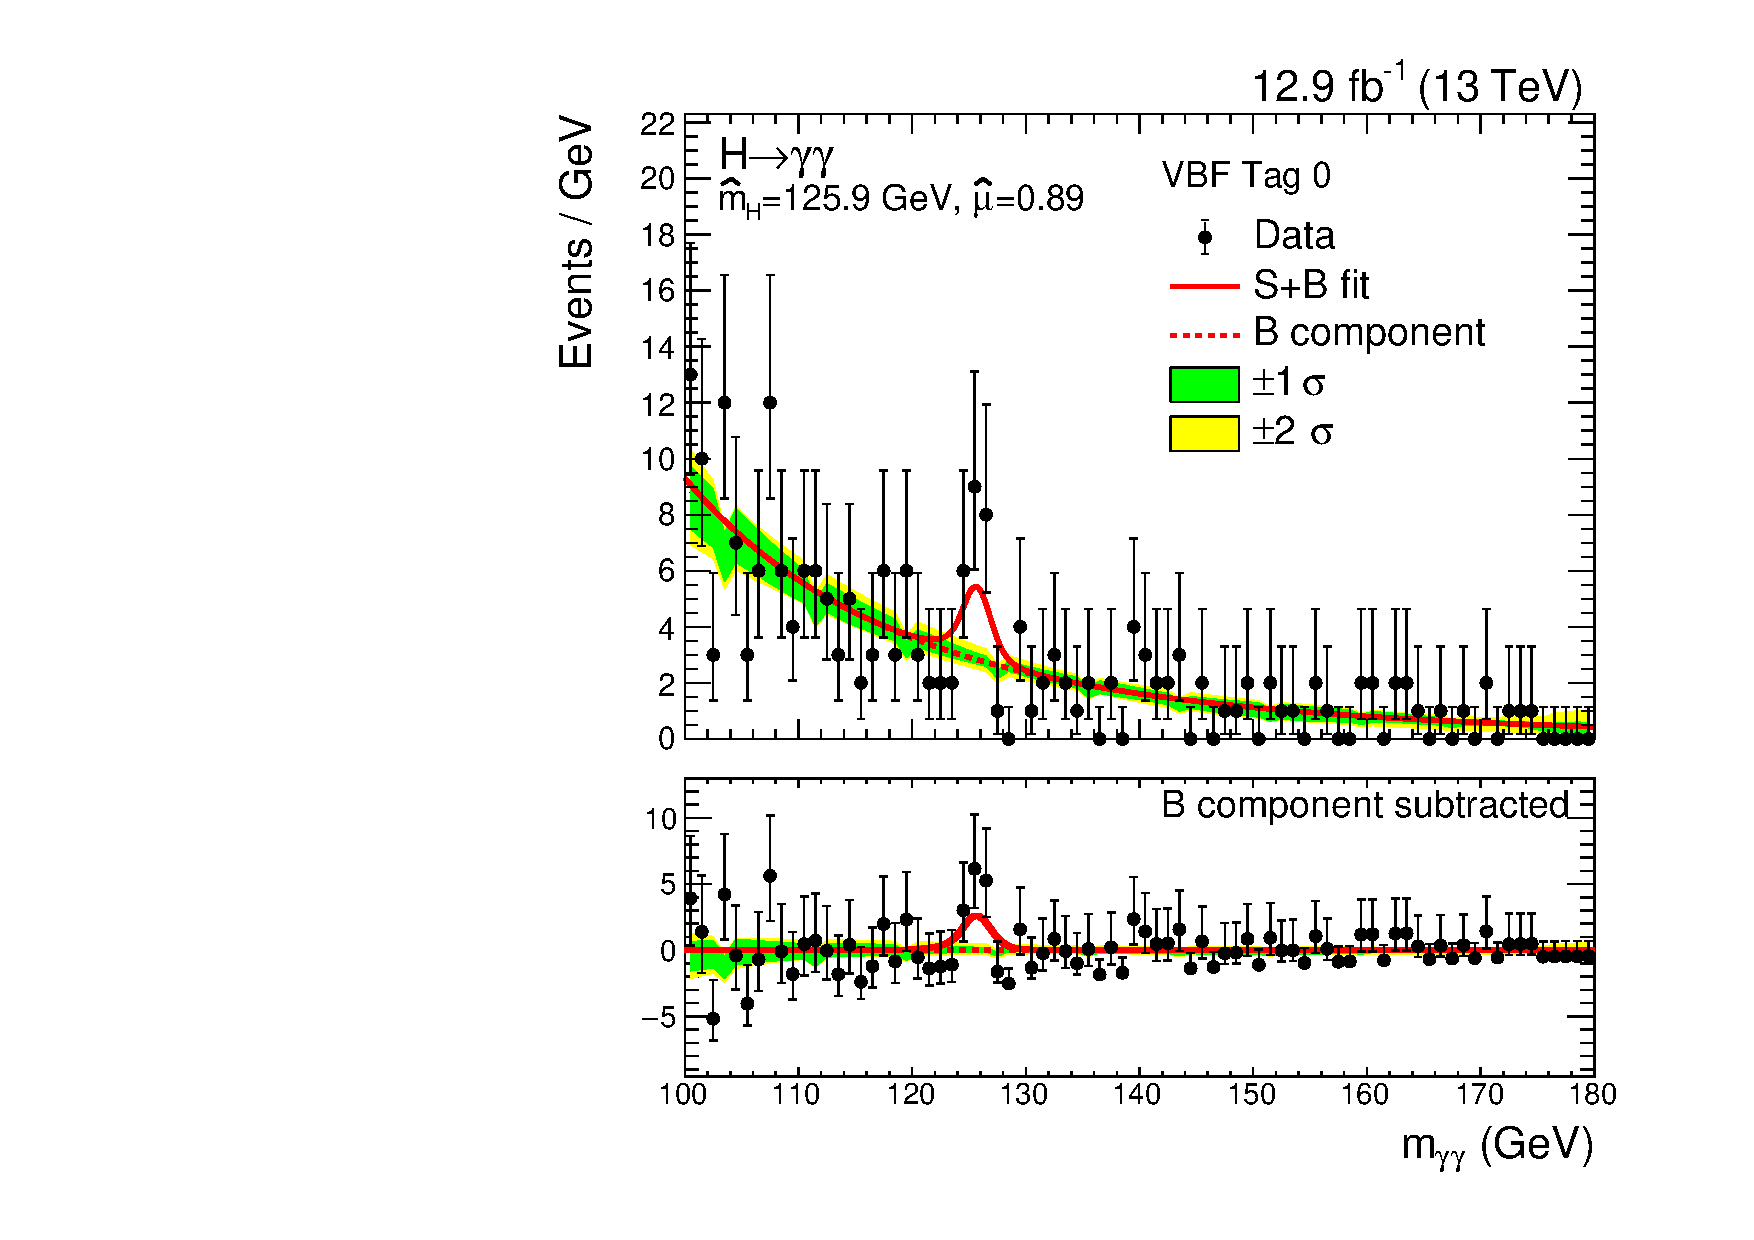
\includegraphics[width=0.49\textwidth]{statandresultsFigures/\whichFig/S_SB_ProfileMH_VBFTag_0_13TeV.pdf} 
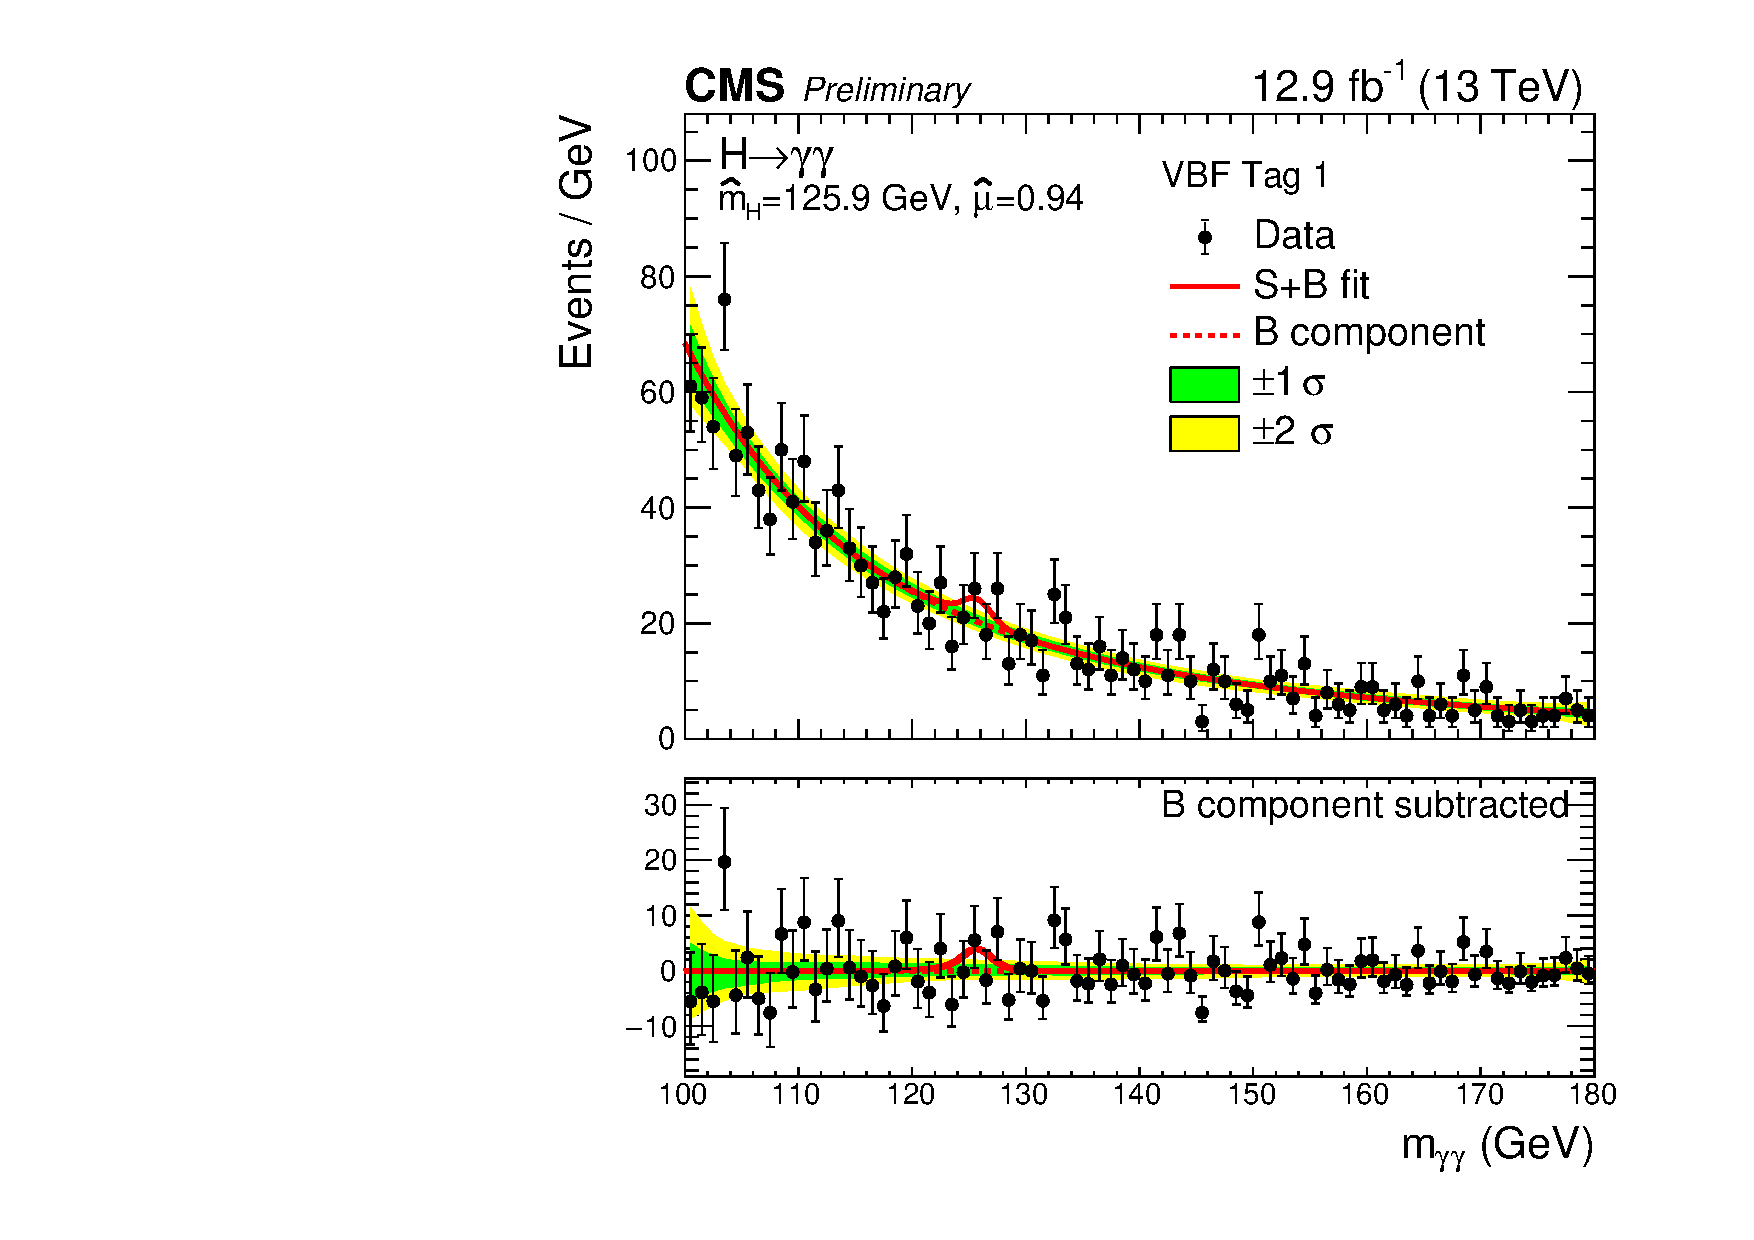
\includegraphics[width=0.49\textwidth]{statandresultsFigures/\whichFig/S_SB_ProfileMH_VBFTag_1_13TeV.pdf} 
%\includegraphics[width=0.3\textwidth]{statandresultsFigures/\whichFig/S_SB_ProfileMH_VBFTag_2_13TeV.pdf} 
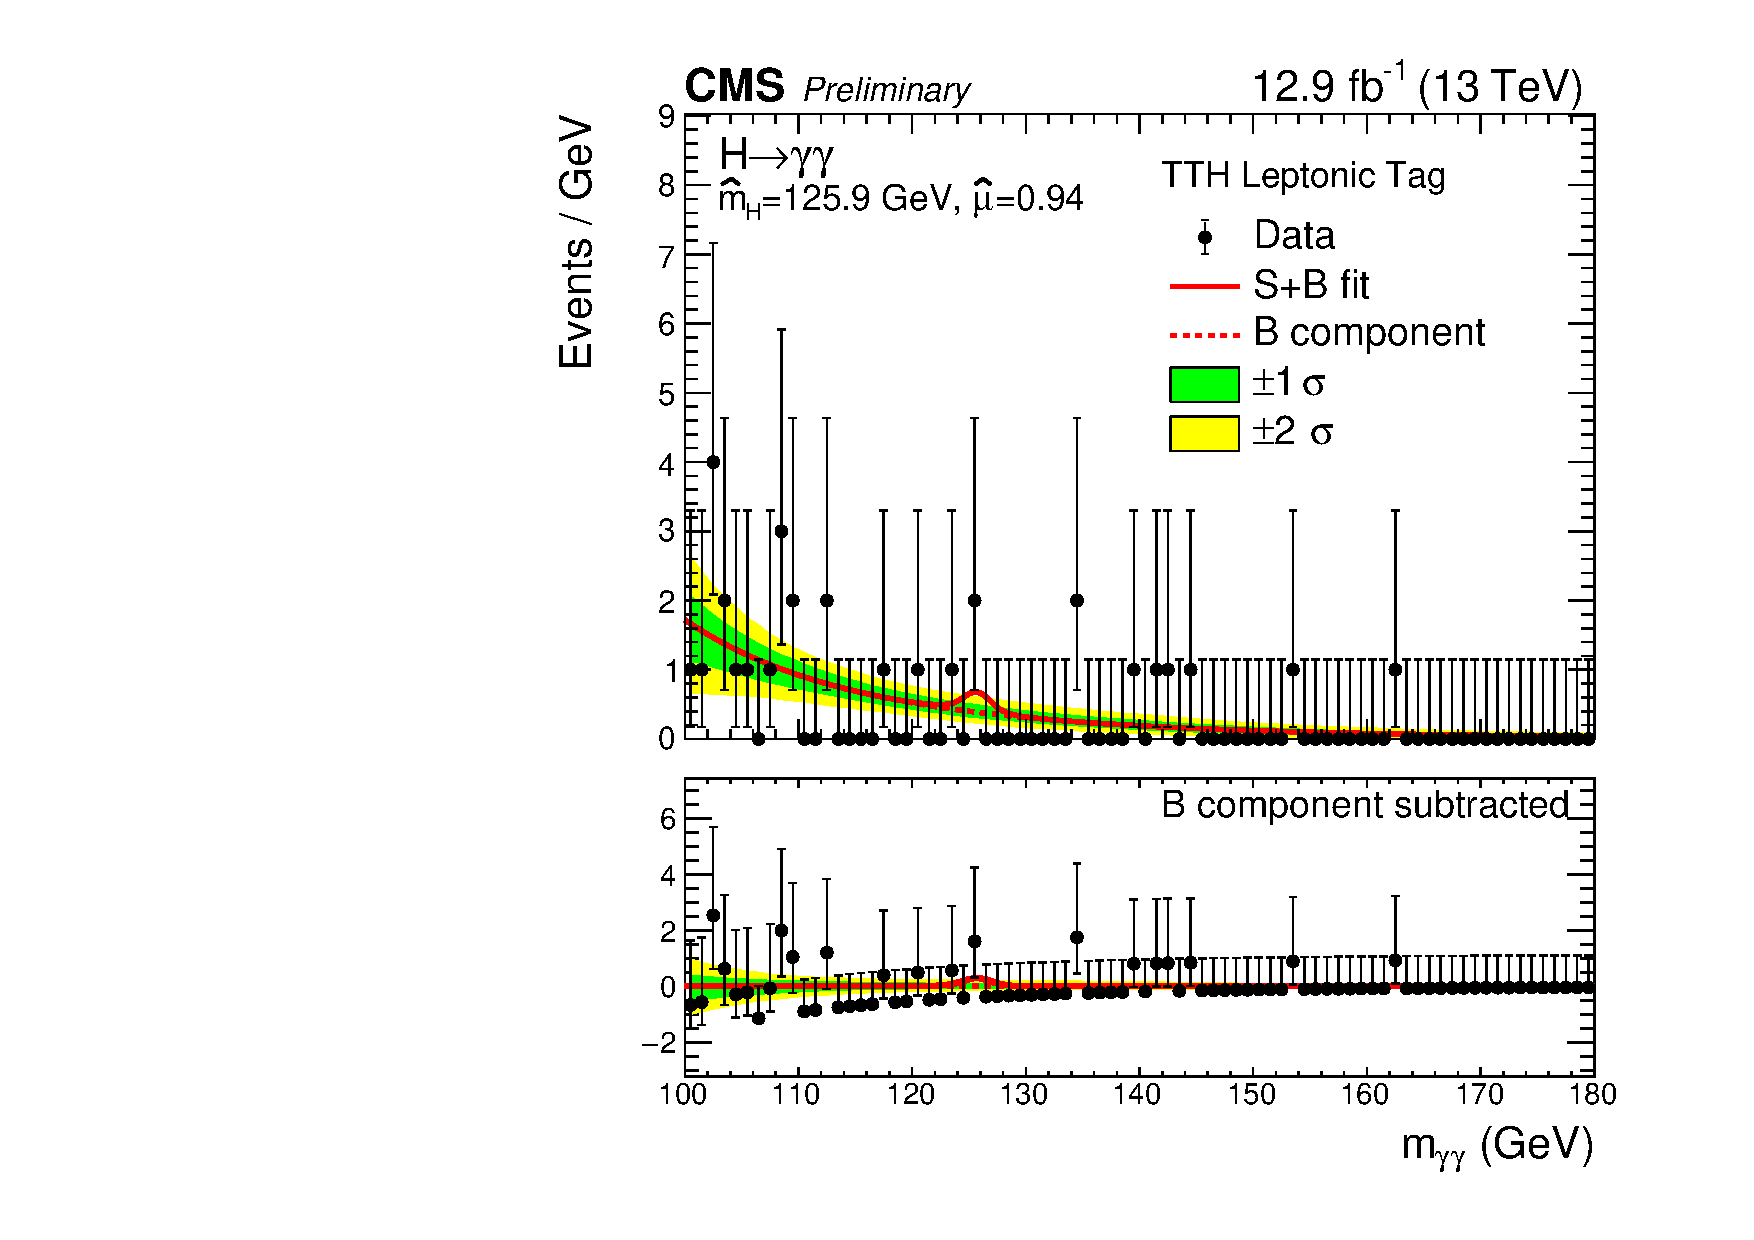
\includegraphics[width=0.49\textwidth]{statandresultsFigures/\whichFig/S_SB_ProfileMH_TTHLeptonicTag_13TeV.pdf} 
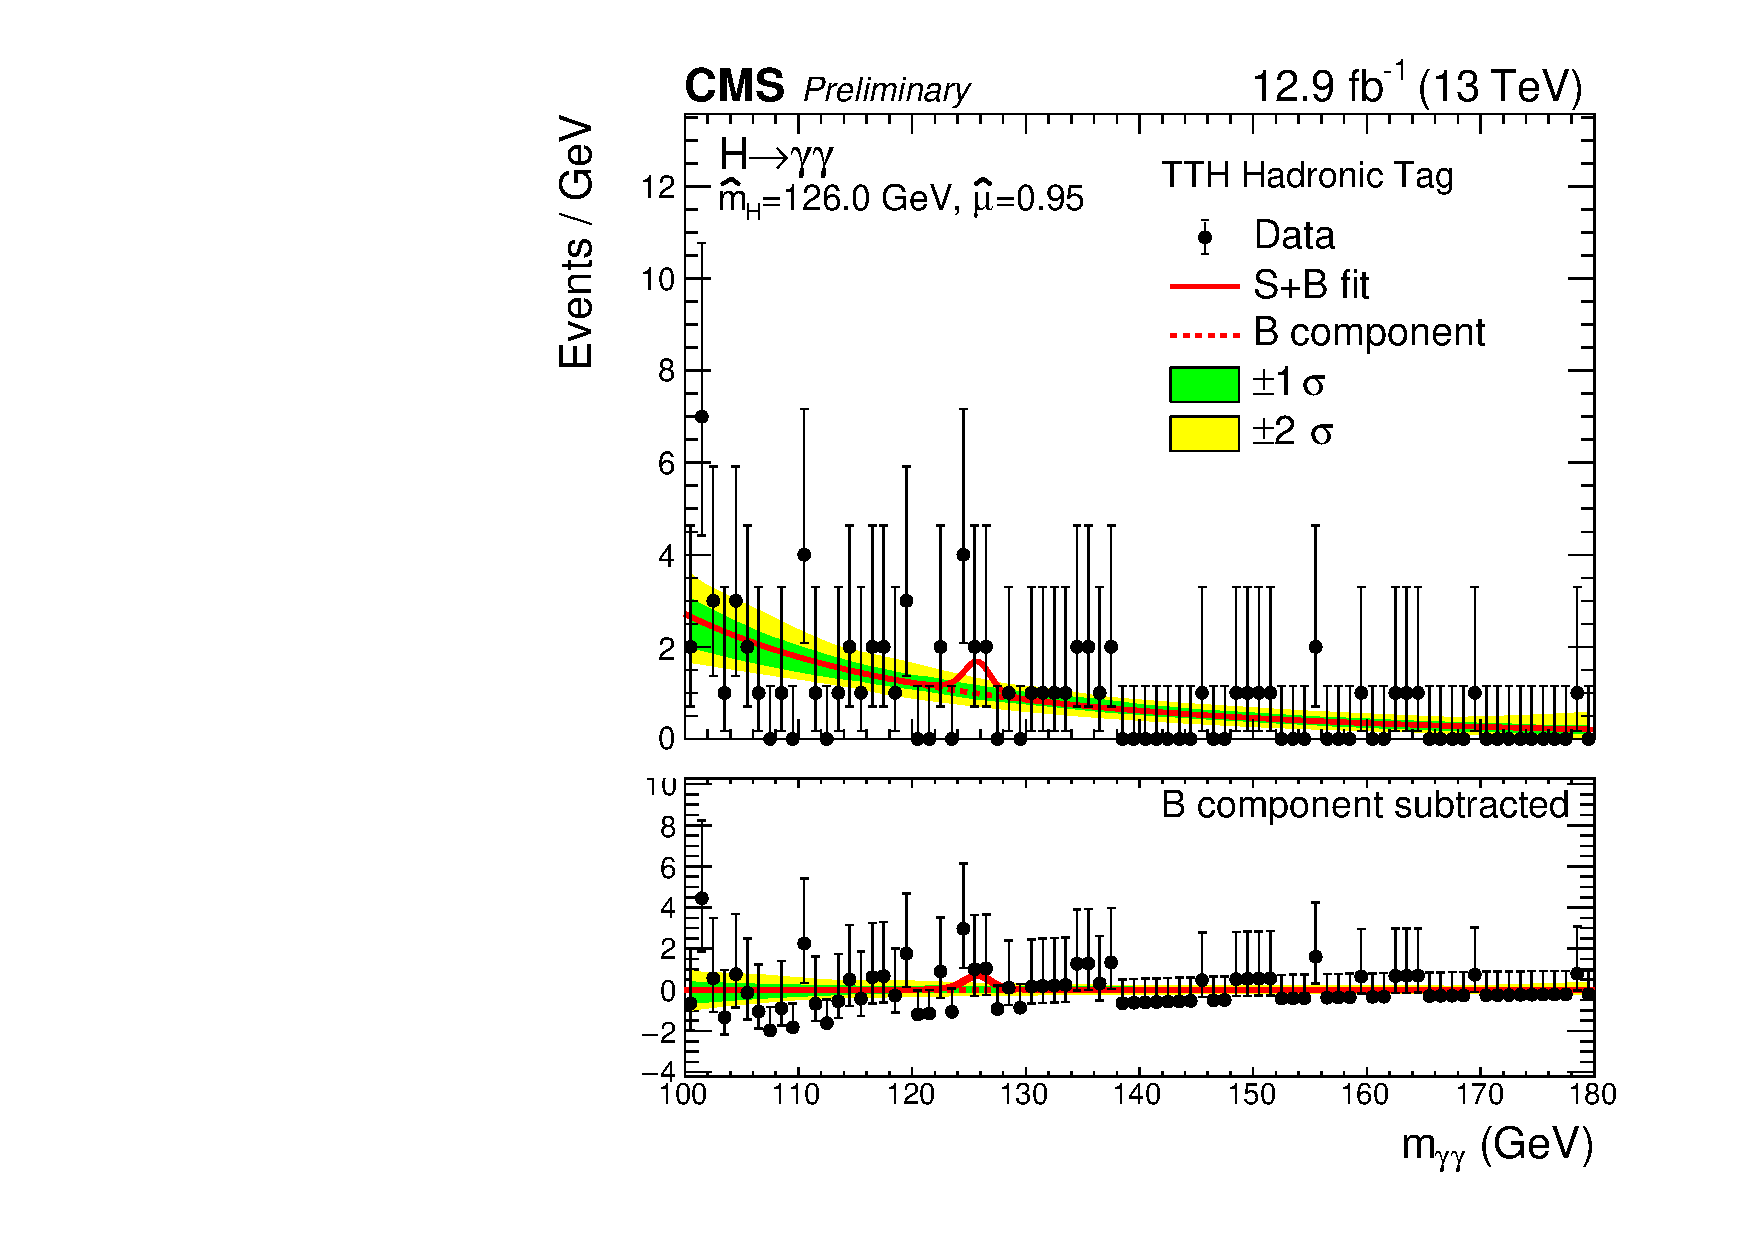
\includegraphics[width=0.49\textwidth]{statandresultsFigures/\whichFig/S_SB_ProfileMH_TTHHadronicTag_13TeV.pdf} \\
%\includegraphics[width=0.3\textwidth]{statandresultsFigures/\whichFig/S_SB_ProfileMH_VHLeptoniclooseTag_13TeV.pdf} 
%\includegraphics[width=0.3\textwidth]{statandresultsFigures/\whichFig/S_SB_ProfileMH_VHMetTag_13TeV.pdf} 
%\includegraphics[width=0.3\textwidth]{statandresultsFigures/\whichFig/S_SB_ProfileMH_VHHadronicTag_13TeV.pdf} \\
%\includegraphics[width=0.3\textwidth]{statandresultsFigures/\whichFig/S_SB_ProfileMH_WHLeptonicTag_13TeV.pdf} 
%\includegraphics[width=0.3\textwidth]{statandresultsFigures/\whichFig/S_SB_ProfileMH_ZHLeptonicTag_13TeV.pdf} 
\caption{The signal-plus-background fit (solid red line) of the observed \mgg distribution in data (black points) for the \VBFTag and \TTHTag analysis categories. The background-only fit is shown as a dashed red line, while the green and yellow bands denote the $1\sigma$ and $2\sigma$ uncertainties on the background shape respectively.}

\label{fig:statandresults:s_b_fits_bis}
\end{figure}

\begin{figure}[hpt!]
\centering
\subfloat[Direct sum]{
 \label{fig:statandresults:s_b_fits_direct_sum}
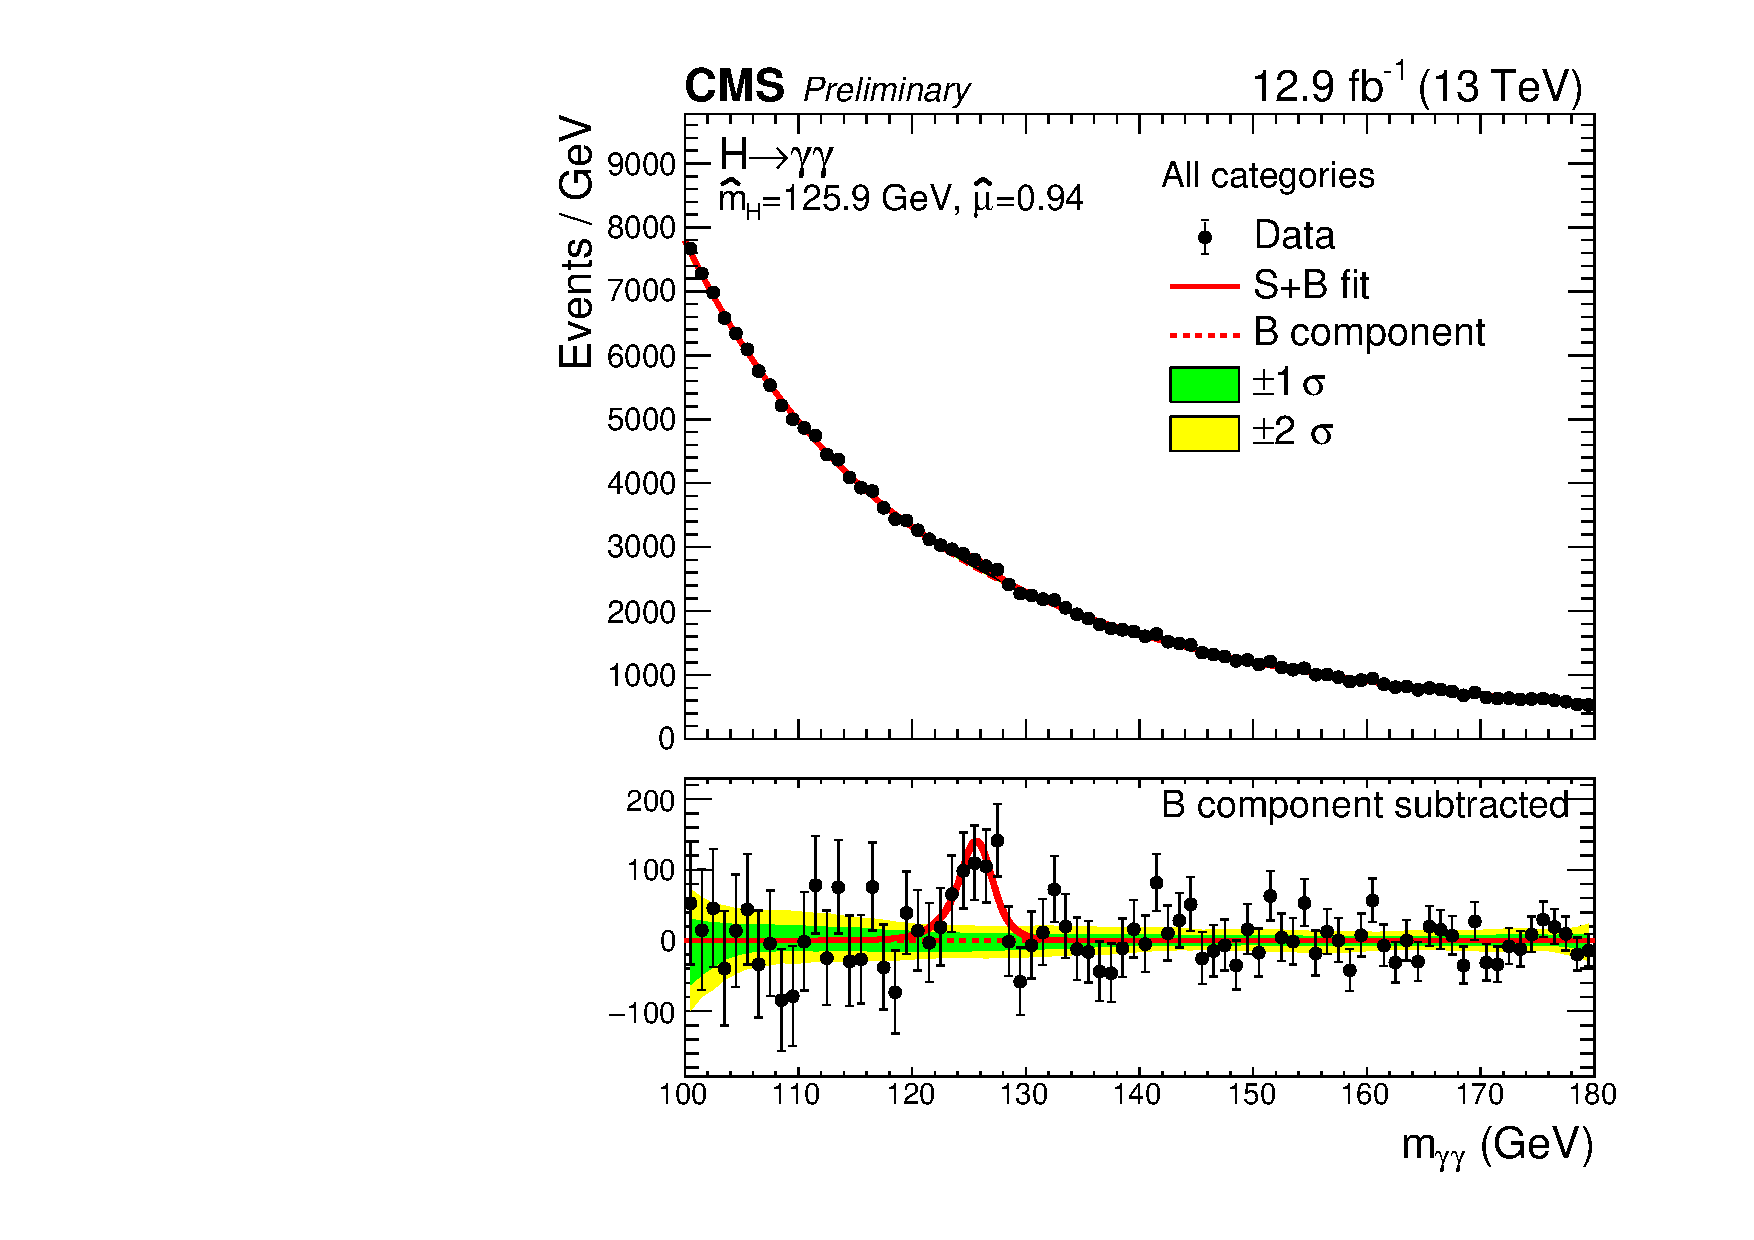
\includegraphics[width=0.59\textwidth]{statandresultsFigures/\whichFig/S_SB_ProfileMH_combcat_unweighted.pdf}}\\
\subfloat[S/(S+B) weighted sum]{
 \label{fig:statandresults:s_b_fits_s_sb_sum}
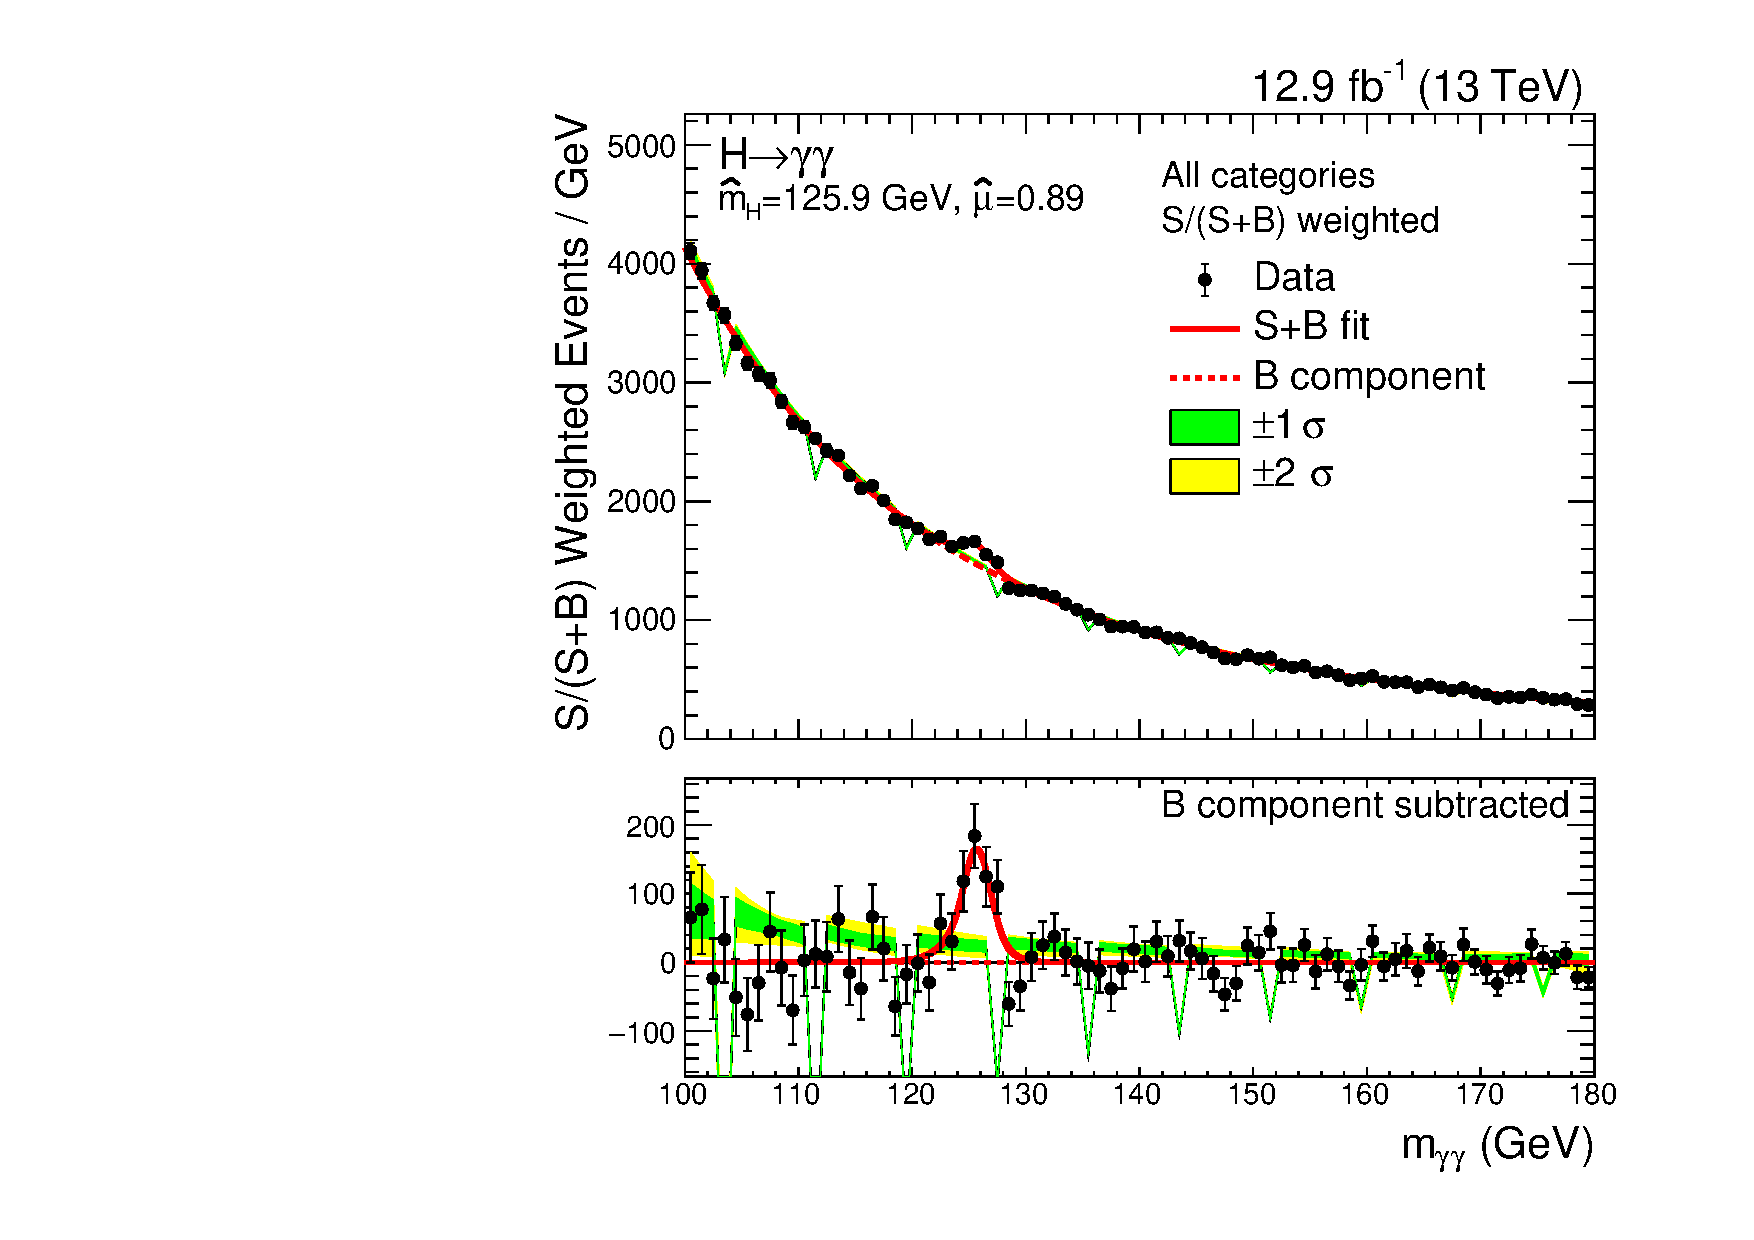
\includegraphics[width=0.59\textwidth]{statandresultsFigures/\whichFig/S_SB_ProfileMH_combcat_weighted.pdf}}
\caption{The signal-plus-background fit (solid red line) of the observed \mgg distribution in data (black points) for all categories combined, either using a direct sum (a) or a sum weighted by the $S/(S+B)$ in $\pm 1 \effSigma$ around the best-fit value of \mH (b). The background-only fit is shown as a dashed red line, while the green and yellow bands denote the $1\sigma$ and $2\sigma$ uncertainties on the background shape respectively.}

\label{fig:statandresults:s_b_fits_sum}
\end{figure}

The best-fit values of the \POI\s are found to be $\hat{\mu}=\bestFitGlobalMu$ and $\hat{\mH}= \bestFitGlobalMH\GeV$ (the best-fit values in~\cite{CMS-PAS-HIG-16-020} were $0.95$ and $126.0$ respectively). The best-fit parametrisation qualitatively indicates the presence of an excess of data in the same place in the \mgg distributions in all analysis categories. When the categories are summed, particularly when weighted by their $S/(S+B)$, the presence of a narrow resonance above the falling background spectrum is visible by eye. The best-fit of the signal-plus-background model to the observed data therefore suggests a \SM-like Higgs boson signal in the data, although a full statistical assessment needs to be undertaken to quantify the size of the excess, taking into account the sources of systematic uncertainty which enter the analysis. 


\section{Significance of observation}
\label{sec:statandresults:significance}

Given the best-fit value of the signal strength $\hat{\mu}= \bestFitGlobalMu$ determined in \Sec~\ref{sec:statandresults:bestfit}, a frequentist approach is used to determine the degree of certainty with which the null hypothesis (that there is no Higgs boson) can be rejected in favour of an alternative hypothesis (that a \SM-like Higgs boson exists). The hypotheses can be formulated in terms of the signal strength: the null hypothesis $H_{0}$ corresponds to the case where $\mu=0$, while the alternative hypothesis $H_{\mu}$ corresponds to $\mu > 0$. 

A statistical test is constructed by specifying a critical region $w$ of the data space, such that for a given set of observed data $\mgg^{obs}$:
\begin{equation}
P(\mgg^{obs} \in w | H_{0} ) \leq \alpha,
\end{equation}
where $P(\mgg^{obs} \in w | H_{0} ) $ is the probability (assuming that $H_{0}$ is correct), of observing the data inside the critical region $w$, and $\alpha$ is a small predetermined threshold~\cite{Cowan}. 

The statistical power $\beta$ of the test is the probability of accepting $H_{0}$ when it is false and the alternative $H_{\mu} $ is true. This is given by:
\begin{equation}
P(\mgg^{obs} \in w | H_{\mu} ) = 1 - \beta.
\end{equation}
The critical region is be chosen such that the power $\beta$ of the test is maximised for a given $\alpha$, to ensure that if $\mgg^{obs} \in w$, then $H_{0}$ has a low probability of being true while $H_{\mu}$ has a high probability of being true. 

A common choice, which is found to maximise $\beta$~\cite{Cowan}, is to define the critical region in terms of a test statistic $q_{\mu}$, corresponding to the difference between the best-fit \NLL and the \NLL (abbreviated as \DNLL) evaluated for a particular $\mu$. The test statistic is defined explicitly as:
\begin{equation}
\label{eq:statandresults:test_statistic}
q_{\mu} = \begin{cases} 
% -2 \ln \mathcal{L}(\mu,\hat{\mH}^{\mu} ; \hat{\mathbf{n}}^{\mu}| \mgg^{obs})- 2\ln\mathcal{L}(\hat{\mu},\hat{\mH} ;\hat{\mathbf{n}}| \mgg^{obs} ) & \text{when } \hat{\mu} \geq 0, \\
 -2 \ln \mathcal{L}(\mu,\mH; \hat{\mathbf{n}}^{\mu}| \mgg^{obs})- 2\ln\mathcal{L}(\hat{\mu},\mH;\hat{\mathbf{n}}| \mgg^{obs} ) & \text{when } \hat{\mu} \geq 0, \\
 0 & \text{when } \hat{\mu} < 0, 
 \end{cases}
\end{equation}

%where $\hat{\mH}^{\mu}$ and 
where $\hat{\mathbf{n}}^{\mu}$ denotes the best fit $\mathbf{n}$ for a fixed value of $\mu$. 
%In this case, \mH is allowed to float with a flat constraint, and is said to be \emph{profiled}. The test statistic can be modified to evaluate the \DNLL for a given \mH hypothesis by fixing it to a particular value instead. 
When trying to exclude hypothesis $H_{0}$, the test statistic $q_{0}$ in particular is used to define a critical region. In the limit of a large sample of data, the probability distribution function of the test statistic ($f_q$), is Gaussian. The fact that $q_{0} =0$ for $\hat{\mu} < 0$ reflects the fact that only excesses in the data are regarded as significant. This simplifies the definition of the critical region, since increasingly large values of $q_{0}$ indicate increasing incompatibility with $H_{0}$, and therefore only the right-hand tail of $f_q$ is considered when assessing probabilities. Assuming $H_{0}$, the probability of obtaining a value of $q^{{obs}}_{0}$ (corresponding to observed data $ \mgg^{obs}$) or higher is given by the integral of $f_q$ from $q^{{obs}}_{0}$ to infinity. This probability is commonly referred to as the \pvalue. We can therefore define the critical region as: 
\begin{equation}
w = \{ \mgg^{obs} : \int_{q^{{obs}}_{0}}^{+\infty} f_q(q_{0}) dq_0 \leq \alpha \},
\end{equation}

In particle physics experiments, the threshold $\alpha$ to reject the null hypothesis is typically $2.87 \times 10^{-7}$. If expressed as the number of standard deviations that a Gaussian-distributed variable would fluctuate to give the same \pvalue, then this threshold is $5\sigma$.

The test statistic $q_{\mu}$ in \Eq~\ref{eq:statandresults:test_statistic} is implicitly defined for a particular assumption on the value of \mH. This ensures that only excesses compatible with the Higgs boson signal distribution for that particular value of \mH are regarded as significant. In other words, only localised excesses in the \mgg spectrum will lead to a small \pvalue. Thus, in this context we refer to local \pvalue\s, which represent the probability that a statistical fluctuation in the observed background distribution gave rise to a localised excess consistent with the signal model at the assumed \mH. The definition of $H_{\mu}$ thus also depends on the assumed value of \mH. In particular, $H_{\mu}$ is the hypothesis that there exists a Higgs boson with mass \mH and signal strength $\mu$. If the observed data fall in the critical region for a given value of \mH, then the null hypothesis (that there is no Higgs boson, regardless of its mass) is rejected in favour of $H_{\mu}$ for that particular \mH. This is not, however, the same as saying that the Higgs boson has that particular value of \mH. The correct statement is that the alternative hypothesis, assuming \mH, is more likely than $H_{0}$ given the data, and that $H_{\mu}$ assuming a different \mH could be yet more likely.

The local \pvalue is therefore evaluated separately, given the observed data, for different assumptions about the value of \mH in the range 120-130\GeV in 0.1\GeV steps. The result is shown in \Fig~\ref{fig:statandresults:pval}. The black solid line represents the local \pvalue scan for the observed data. The dashed lines represent the expected local \pvalue\s for a \SM Higgs boson. These are obtained by generating an Asimov dataset~\cite{Cowan:2010js} from the best-fit background-only model and a signal of strength $\mu=1$, and then performing a signal-plus-background fit and following the same procedure as for observed data. For the blue dashed line, the signal was injected at $\mH=125.09\GeV$ (the best fit value from the previous combined \RunI measurement by \CMS and \ATLAS~\cite{PhysRevLett.114.191803}), while for the red dashed line the signal was injected at the corresponding \mH for each step. 


\begin{figure}[ht!]
\centering
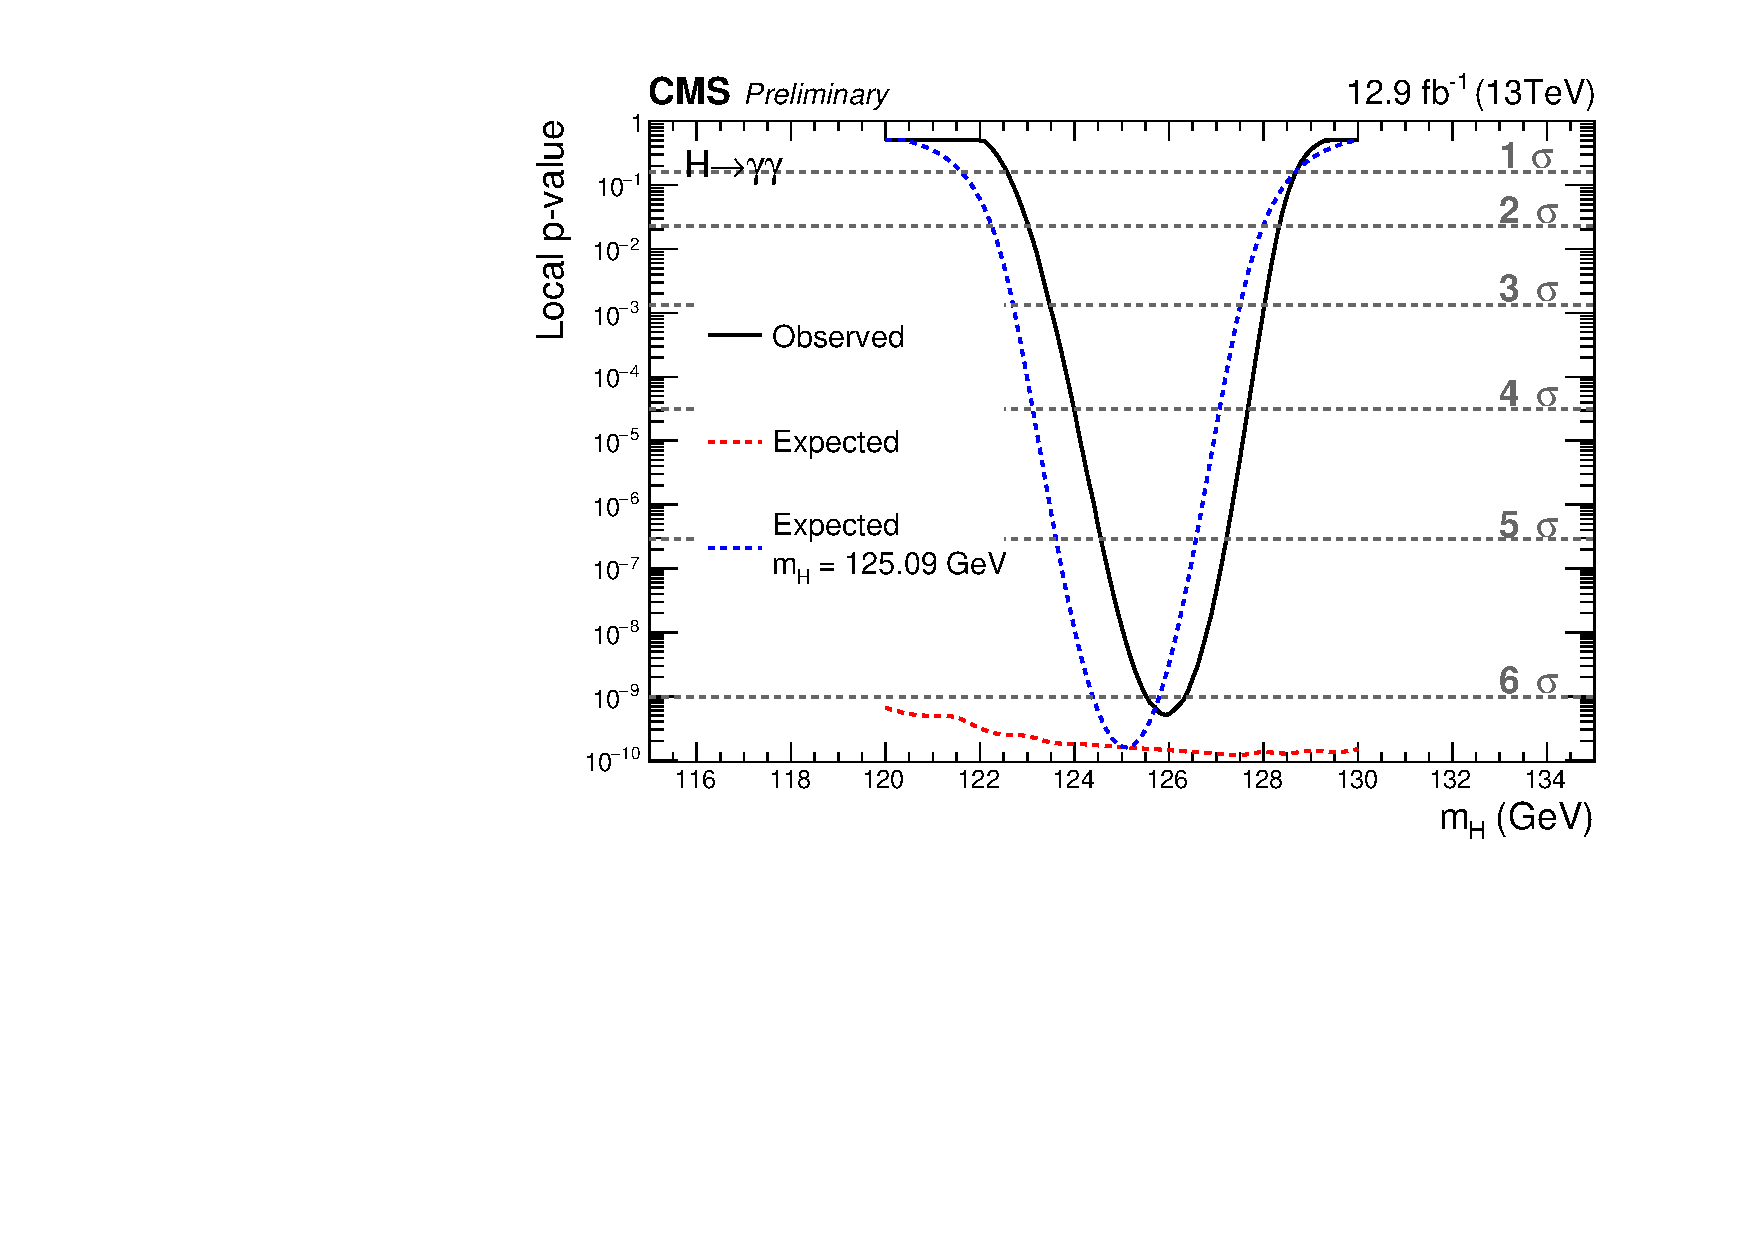
\includegraphics[width=0.9\textwidth]{statandresultsFigures/\whichFig/pval13TeV-observed.pdf} 
\caption{The local \pvalue for the observation as a function of the Higgs boson mass (black), shown with the expected local \pvalue\s for a SM Higgs boson, across the range 120-130\GeV. The expected local \pvalue\s are obtained using Asimov datasets. The blue dashed line shows the expected local \pvalue when the mass of the injected signal is $\mH=125.09\GeV$, while the red line shows the maximum significance for any injected signal in the range of $120$ to $130\GeV$.}

\label{fig:statandresults:pval}
\end{figure}

The local observed significance at the \RunI best fit ($\mH=125.09\GeV$) is $\obsSigAtRunIBF\sigma$, where $\expSigAtRunIBF\sigma$ was expected for the \SM Higgs boson. The maximum local observed significance is found at $\bestFitGlobalMH\GeV$, corresponding to $\obsSigAtMin\sigma$ where $\expSigAtMin\sigma$ was expected (these results are consistent with~\cite{CMS-PAS-HIG-16-020} to within one unit of the smallest quoted decimal place). % $5.6\sigma$ at $\mH=125.09\GeV$ is where $6.2\sigma$ was expected, and maximum local observed significance at $\mH=126.0\GeV$, corresponding to $6.1\sigma$.
Since the observed data fall in the critical region where at least one \mH assumption yields a local significance above $5\sigma$ (i.e \pvalue is less than $2.87 \times 10^{-7}$), the null hypothesis that there is no Higgs boson is rejected in favour of the alternative hypothesis that there exists a Higgs boson. Therefore, the data correspond to an observation of the Higgs boson decaying to photons.

The maximum significance of the observation in this analysis occurs near $\mH=126.0\GeV$, which is somewhat different from the combined best-fit \mH measured in \RunI. %world average values of $125.09\pm0.24\GeV$ from the combination of \CMS and \ATLAS results from \RunI ~\cite{PhysRevLett.114.191803}. 
However, the results which are presented here do not comprise a measurement of the Higgs boson mass, as the data were not reprocessed with the final set of \ECAL calibrations and tuning of the \PhoEnergyBdt which are required for a precision measurement. %As can be seen from \Table~\ref{tab:model:systematics}, the corresponding shape nuisances have a negligible effect on the measurements of the signal strength and related quantities, and therefore these considerations do not invalidate the results presented in this thesis.

\section{Measurements of the signal strength}
\label{sec:statandresults:sigstrength}
\subsection{Global signal strength}
\label{sec:statandresults:sigstrength_global}

One of the advantages of using \DNLL as a test statistic is that to a very good approximation, the $\pm 1 \sigma$ and $\pm 2 \sigma$ uncertainty on the measured value of a \POI can be obtained by finding the values of the \POI for which $\DNLL=1$ and $\DNLL=4$ respectively~\cite{Cowan}. %$q_{\mu}=q_{\hat{\mu}}+1$~\cite{Cowan}.
This fact is used to produce a measurement of the global signal strength $\mu$. 

Two modifications are made to the definition of the test statistic in \Eq~\ref{eq:statandresults:test_statistic}. First, the \mH parameter is profiled in the minimisation at each step, which means that it is allowed to float with a flat constraint. Second, the requirement that the test-statistic is nonzero only for positive values of $\hat{\mu}$ is relaxed, since this was a enforced to simplify the calculation of \pvalue\s. The new definition of the test statistic is therefore given by: 
\begin{equation}
\label{eq:statandresults:test_statistic_profMH}
q_{\mu} = -2 \ln \mathcal{L}(\mu,\hat{\mH}^{\mu} ; \hat{\mathbf{n}}^{\mu}| \mgg^{obs})- 2\ln\mathcal{L}(\hat{\mu},\hat{\mH} ;\hat{\mathbf{n}}| \mgg^{obs} ), 
\end{equation}
where $\hat{\mathbf{\mH}}^{\mu}$ denotes the best-fit \mH for a fixed value of $\mu$. %Other treatements of the \mH paramater are possible (for instance, fixing it to the central value from the current best measurement, or Gaussian-constraining it within the uncertainties of the best measurement), but these do not signifiancelty change the final measurement of the signal strength.

The measurement is made by evaluating the test statistic for fixed values of $\mu$ in small steps in the range of $0.5$ to $1.5$. The result of the so-called \DNLL \emph{scan} of $\mu$ is shown in \Fig~\ref{fig:statandresults:global_mu}. By definition, the best-fit point $\hat{\mu}$ has a \DNLL value of $0$. This gives the central value for the measurement. The upper and lower uncertainties are obtained by finding the intercepts of the curve with \DNLL$=1$. 
The contribution to the total uncertainty on the signal strength arising from the statistical, experimental systematic and theory systematic components are assessed by repeating the process, but freezing the corresponding nuisance parameters to their post-fit values. Their effect is then calculated by taking the difference in quadrature with respect to the total uncertainty. 
The measured value of the signal strength is:
\begin{equation*}
\obsMuBreakdown,
%\hat{\mu}=0.95 ^{+0.21}_{-0.19} = 0.95 \pm 0.17 \text{ (stat.) }^{+0.09}_{-0.06} \text{ (theo. syst.) }^{+0.10}_{-0.07} \text{ (exp. syst.)}. 
\end{equation*}
which is consistent with the result quoted in~\cite{CMS-PAS-HIG-16-020} to within one decimal place. 

This measurement indicates that the observed global signal strength is compatible with the \SM expectation within one standard deviation. The observed particle therefore appears to behave very closely to the predictions of the \SM in its overall production rate. None, the less, various extensions to the \SM predict variations of the order of a few percent, and therefore the current uncertainties, which are of the order of $20\%$, cannot rule out contributions from physics beyond the \SM. Further accumulation of data during the \LHC programme will help to bring down this uncertainty, which is currently dominated by the statistical component. The full 2016 dataset contains approximately three times as much data, which would already be enough to bring the statistical contribution to the uncertainty to the level of the theory and experimental systematic contributions.

A similar likelihood scan can be repeated for specific values of \mH in the 120-130\GeV range, using the \DNLL definition from \Eq~\ref{eq:statandresults:test_statistic} but removing the requirement that the test-statistic is nonzero only for positive values of $\hat{\mu}$.
The result is shown in \Fig~\ref{fig:statandresults:mu_vs_mh}, where the best-fit signal strength is plotted as a function of the fixed value of \mH in 0.1\GeV steps. The green bands represent the $\pm 1 \sigma$ uncertainty obtained by finding the crossing with \DNLL$=1$ for each step. This figure illustrates that no excesses other than the one at the best-fit exist in the region of interest. %An interesting feature of this plot is that the value of $\hat{\mu}$ at the edges is found to be consistently negative. This is because the effect of the excess measured in data near $\bestFitGlobalMH$\GeV on the background-only fit.

\begin{figure}[ht!]
\centering
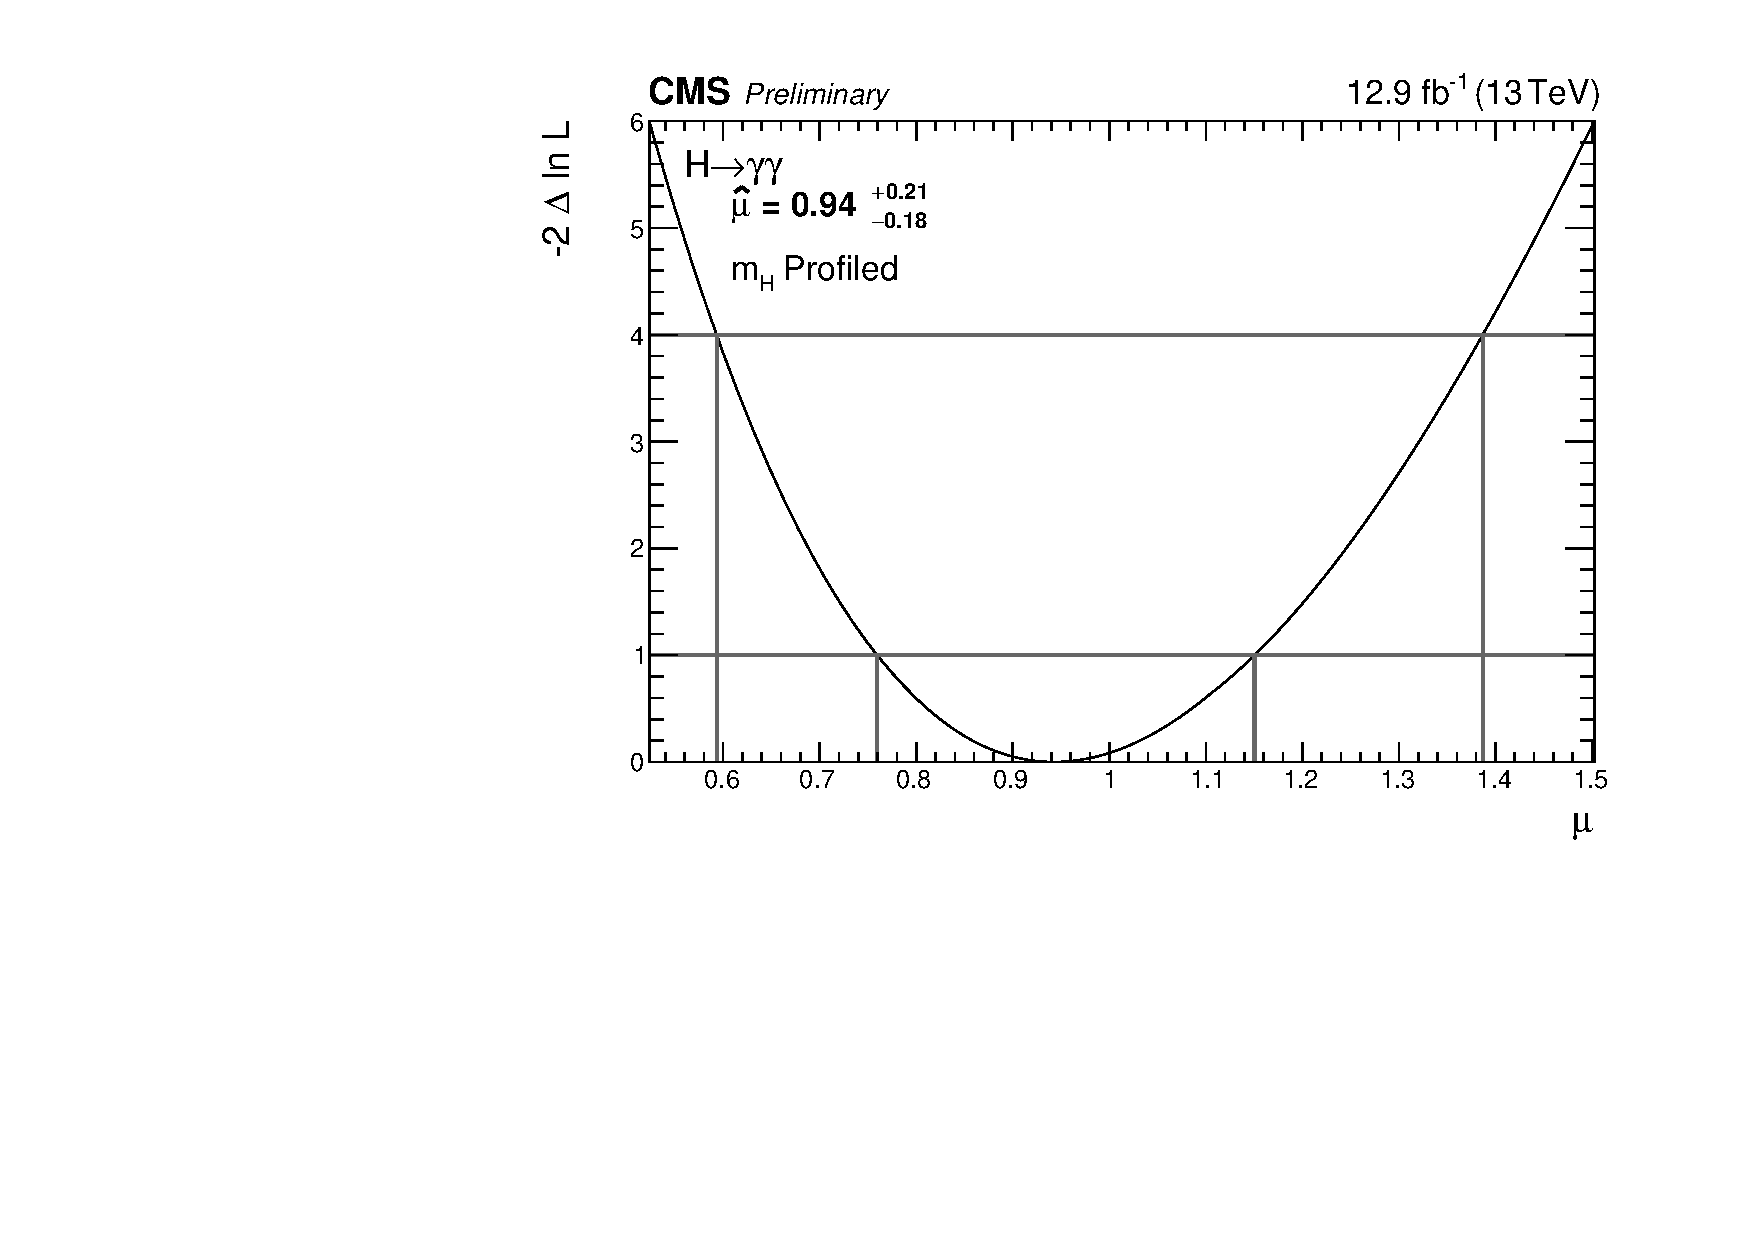
\includegraphics[width=0.9\textwidth]{statandresultsFigures/\whichFig/MuScanProfileMH.pdf} 
\caption{The \DNLL scan of the overall signal strength for a Higgs boson decaying to two photons. The mass of the Higgs boson is profiled in the fit. The $1\sigma$ and $2\sigma$ uncertainties correspond to the crossings with \DNLL$=1$ and \DNLL=$4$.}

\label{fig:statandresults:global_mu}
\end{figure}


\begin{figure}[ht!]
\centering
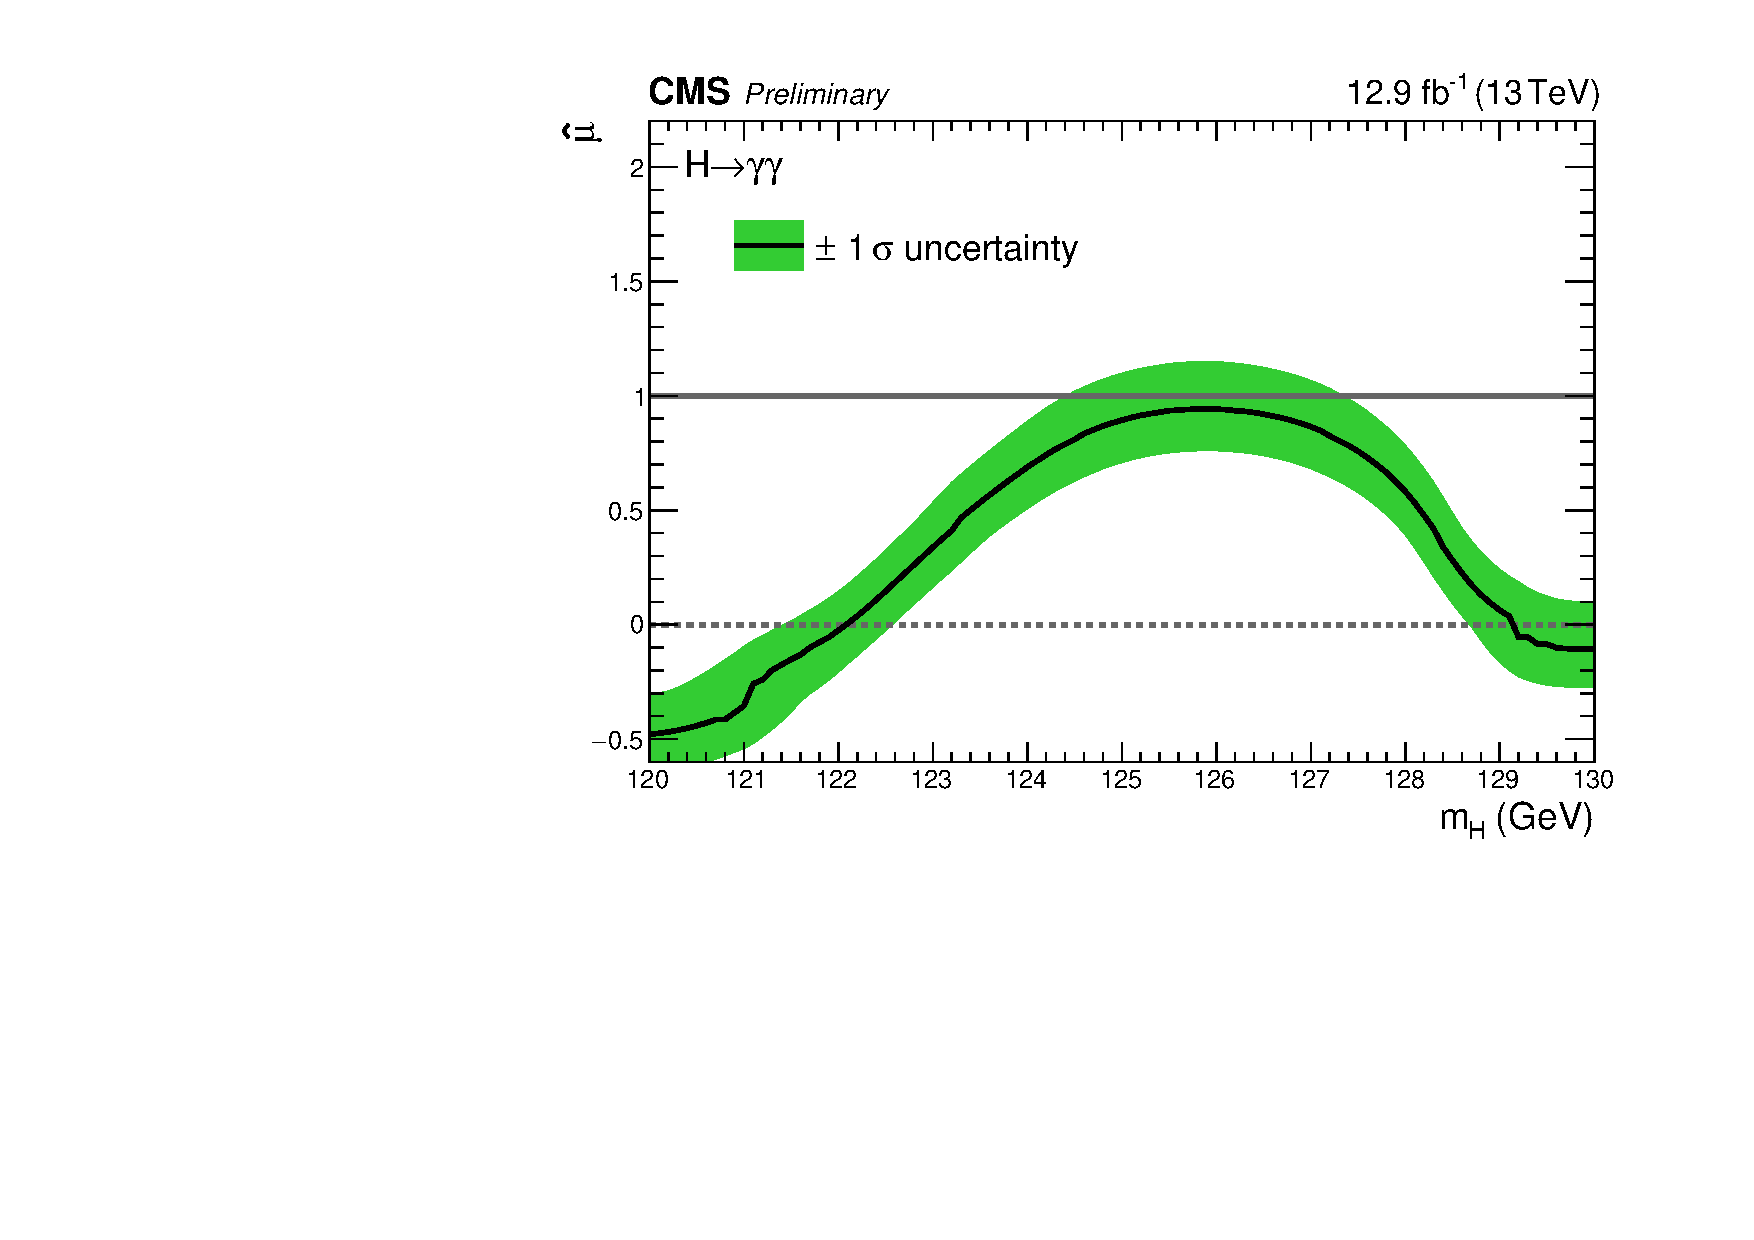
\includegraphics[width=0.9\textwidth]{statandresultsFigures/\whichFig/MuHat_vs_MH.pdf} 
\caption{The best-fit signal strength for fixed values of \mH in the 120-130\GeV range, where the \mH parameter is fixed in the fitting procedure. The green bands show the $\pm 1 \sigma$ uncertainty obtained by finding the crossing with \DNLL$=1$. }

\label{fig:statandresults:mu_vs_mh}
\end{figure}

\subsection{Fermionic and bosonic components of the signal strength}
\label{sec:statandresults:rvrf}

When making the measurement of the global signal strength as in \Sec~\ref{sec:statandresults:sigstrength_global}, a single \POI which uniformly scales all production processes in all categories is defined. However, this measurement makes the assumption that the contribution of each production process to the total Higgs boson \crosssection is in proportion to the \SM prediction. 
In order to test this assumption, the single \POI representing to global signal strength can be split up into components. For example, the contributions from the production modes where the Higgs boson is produced from fermions (\ggH and \ttH) and vector bosons (\VBF and \VH) are separated, to test if they individually agree with the \SM expectation. 

A modified likelihood function is required, which is amended from \Eq~\ref{eq:statandresults:likelihood_function} to include two \POI\s, \muF and \muV in the place of $\mu$:
\begin{equation}
\label{eq:statandresults:likelihood_function_muVmuF}
\begin{split} 
\mathcal{L}(\muF, \muV,{}& \mH; \mathbf{n} | \mgg^{obs} ) = \prod_{C} \big[ f^C_B(\mgg^{obs,C} | \mathbf{n}_B )   \\
& +\muF \cdot ( f^C_{S,{\text{ggH}}}(\mgg^{obs,C} |\mH ; \mathbf{n}_S) + f^C_{S,{\text{ttH}}}(\mgg^{obs,C} |\mH ; \mathbf{n}_S) ) \\ 
& +\muV \cdot ( f^C_{S,{\text{VBF}}}(\mgg^{obs,C} |\mH ; \mathbf{n}_S) + f^C_{S,{\text{VH}}}(\mgg^{obs,C} |\mH ; \mathbf{n}_S) )\big].
 \end{split} 
\end{equation}
%In the definition above, $f^C_{S,{\text{ggH}}}$, $f^C_{S,{\text{ttH}}}$, $f^C_{S,{\text{VBF}}}$ and $f^C_{S,{\text{VH}}}$ represent the probability distribution functions of the signal models resulting from each production process, as defined in \Eq~\ref{eq:statandresults:f_s_breakdown}.
In this new likelihood function, the \muF parameter scales the yield of the signal models for \ggH and \ttH in all categories uniformly, but does not affect the yields of the models for \VBF or \VH, and vice versa for the \muV parameter.
%The full likelihood $\mathcal{L}$ is then obtained by taking the product of the likelihood functions in each category.

The measurement is made by producing a two-dimensional \DNLL scan. The test statistic $q_(\muF,\muV)$ is defined as in \Eq~\ref{eq:statandresults:test_statistic_profMH} (i.e. with \mH profiled), but using the amended definition of the likelihood from \Eq~\ref{eq:statandresults:likelihood_function_muVmuF}. 
The result of the two-dimensional scan can be seen in \Fig~\ref{fig:statandresults:mu_per_rvrf}. 
%The $z$-axis, representing the value of \DNLL, has been omitted for clarity. 
The black cross shows the location of the best-fit point, with the red diamond indicating the \SM expectation. In two-dimensional \DNLL scans, the $1\sigma$ and $2\sigma$ contours are the intersections with $\DNLL=2.30$ and $\DNLL=6.18$ respectively~\cite{Cowan}, and these are shown as solid and dashed lines in the figure. 

The plot shows that the observed best-fit point is consistent with the \SM within $1\sigma$. The elliptical shape of the contours reflects the fact that the \Untagged categories, which are by far the most sensitive due to their high event content and $S/(S+B)$, are populated chiefly by \ggH events. This results in a strong constraint on the \muF parameter, and a somewhat looser one on the \muV parameter. The uncertainty ellipses are also slightly inclined, which can be understood by the fact that the \VBF-targeting categories contain a non-negligible amount of \ggH events, and vice-versa. This leads to slight correlation: an increase in \muF typically must come at the expense of a decrease in \muV to ensure a good fit in all analysis categories.


\begin{figure}[ht!]
\centering
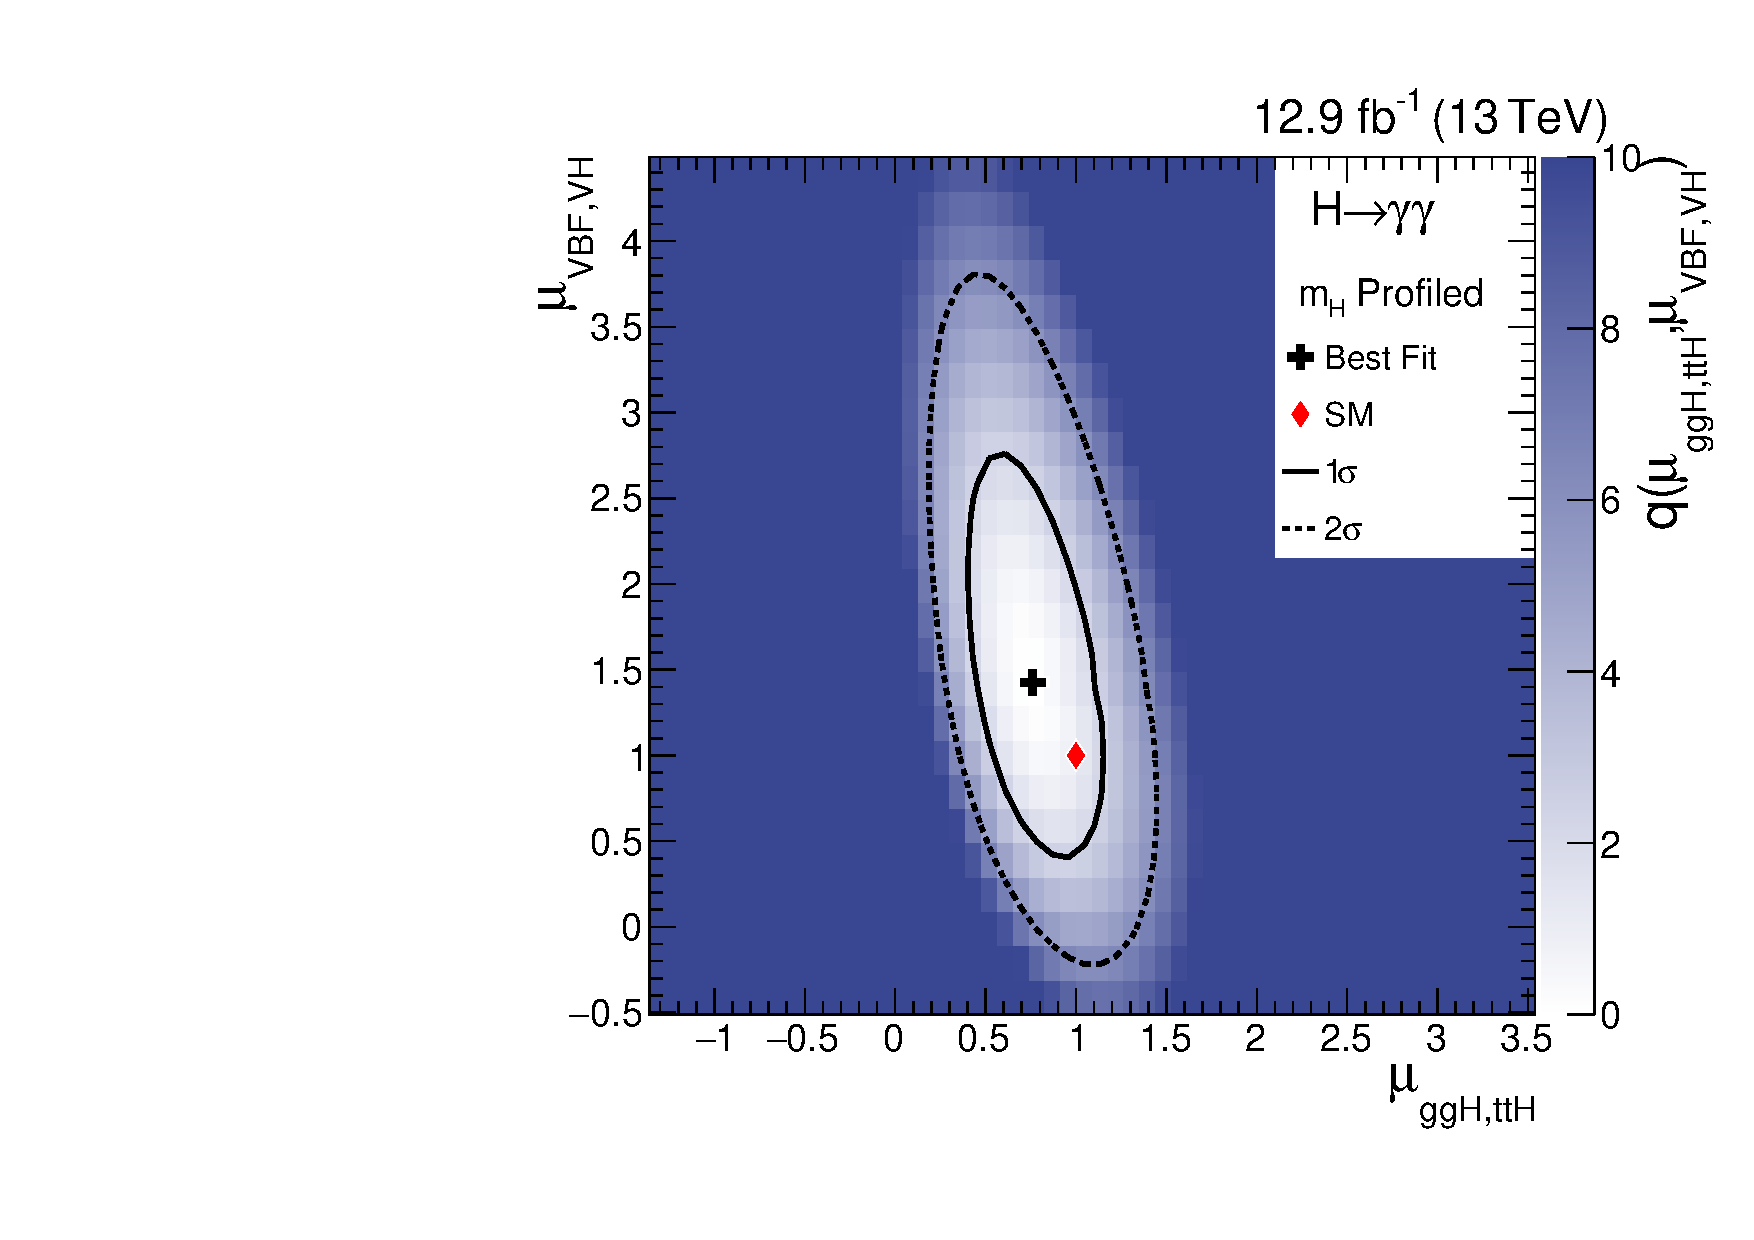
\includegraphics[width=0.8\textwidth]{statandresultsFigures/\whichFig/RVRFScanProfileMH_col.pdf} 
\caption{The result of a two-dimensional \DNLL scan of the \muF and \muV components of the signal strength. The red diamond indicates the SM expectation, while the black cross shows the location of the best-fit point. The measurement is consistent with the SM within the uncertainty contours, which are shown in solid and dashed lines for the $1\sigma$ and $2\sigma$ uncertainties respectively. The value of \mH was profiled in the scan.}

\label{fig:statandresults:mu_per_rvrf}
\end{figure}

To correctly extract the uncertainties on  the \muF and \muV parameters individually, a \DNLL scan of each is performed while profiling the other. This is achieved by modifying the test statistic to treat the profiled \POI analogously to \mH in \Eq~\ref{eq:statandresults:test_statistic_profMH}. 

The resulting scans are available in \App~\ref{app:dnll_scans} in \Fig~\ref{fig:statandresults:mu_per_rv_and_rf}, which give rise to the following measurements:
\begin{equation*}
%\muFhat=0.82^{+0.27}_{-0.24} \text{ and } \muVhat=1.60^{+0.90}_{-0.76}.
\begin{split}
\obsMuV, \\
\obsMuF.
\end{split}
\end{equation*}

The \muF measurement is consistent with~\cite{CMS-PAS-HIG-16-020} to within one unit of the smallest quoted decimal place and \muV differs by less than $5\%$ which is small compared to the size of the uncertainties. The fermionic and bosonic components of the signal strength are therefore each found to be individually compatible with the \SM expectations. %As expected, the component related to the \ggH production mode has by far the smallest uncertainties, since it exerts the most influence on the fit in the sensitive \Untagged categories.

%\newpage

\subsection{Per-process signal strengths}
\label{sec:statandresults:mu_per_proc}

Using a similar procedure to that described in \Sec~\ref{sec:statandresults:rvrf}, measurements of the signal strengths of the individual Higgs boson production modes can be made. In this case, the likelihood function and test statistic are modified to contain one \POI for each production process (\muggH, \muVBF, \muVH, and \muttH). Each per-process signal strength independently scales the yield for the signal models for the corresponding process in all categories, leaving the signal models for the other processes unchanged. The likelihood function for is therefore defined as:
\begin{equation}
\label{eq:statandresults:likelihood_function_muProc}
\begin{split}
\mathcal{L}(\muggH, \muttH,\muVBF,\muVH, \mH; \mathbf{n} | \mgg^{obs} ) = \prod_C \big[{} &f^C_B(\mgg^{obs,C} | \mathbf{n}_B ) \\ 
&+\muggH\cdot f^C_{S,{\text{ggH}}}(\mgg^{obs,C} |\mH ; \mathbf{n}_S) \\ 
&+\muttH\cdot f^C_{S,{\text{ttH}}}(\mgg^{obs,C} |\mH ; \mathbf{n}_S) \\ 
&+\muVBF\cdot f^C_{S,{\text{VBF}}}(\mgg^{obs,C} |\mH ; \mathbf{n}_S) \\
&+\muVH \cdot f^C_{S,{\text{VH}}}(\mgg^{obs,C} |\mH ; \mathbf{n}_S){}\big], \\ 
\end{split}
\end{equation}
The technique described above exploits the categorisation scheme described in \Chapter~\ref{chap:categorisation}: in particular, the fact that the relative contribution from each process to the overall signal model differs from category to category. This means that varying each per-process signal strength has a different effect on the overall likelihood function. However, since no \VHTag categories are included in this analysis, it is not possible to resolve the effect of varying \muVH from other \POI\s, in particular \muggH, since most \VH events are included in the \Untagged categories along with the \ggH events. To break the degeneracy, when making the measurements of the other \POI\s, the parameter \muVH is fixed to a value of 1. 

The measurements of the \muggH, \muVBF, and \muttH are performed by producing a \DNLL scan of each parameter, while profiling the others, where the \DNLL definition has been suitably modified to accommodate the new likelihood function defined in \Eq~\ref{eq:statandresults:likelihood_function_muProc}. The \mH parameter is also profiled. The best-fit values and their uncertainties are shown on \Fig~\ref{fig:statandresults:mu_per_proc}. The measurement of the global signal strength obtained in \Sec~\ref{fig:statandresults:global_mu} is shown as the vertical black line with green bands showing the $1\sigma$ uncertainties. The \SM expectation is shown as the vertical dashed red line. The per-process signal strength measurements are all compatible with the \SM expectation within $1\sigma$. The measurements also agree with those presented in~\cite{CMS-PAS-HIG-16-020} within one unit of the smallest significant figure for \muggH, and within $5\%$ for \muVBF and \muttH, which is small compared to the $1\sigma$ uncertainties. 

This result is of particular interest because certain extension to the \SM predict modified values of the per-process signal strengths. In particular, if a heavy top-like particle exists (as predicted by many theories to resolve the hierarchy problem), then an anomalous value of $\muttH$ could be observed. However, the variations in the value of \muttH predicted by such models are typically smaller than 10\%. There is evidently plenty of room to accommodate such variations in the current measurement. As more data are collected over the course of the \LHC programme, this type of measurement will become increasingly important since it could reveal clues to the nature of physics beyond the \SM, or put strong constraints on proposed extensions. This result also shows that the bulk of the sensitivity of the analysis resides in the \Untagged categories, which are largely composed of \ggH events.

\begin{figure}[h!]
\centering
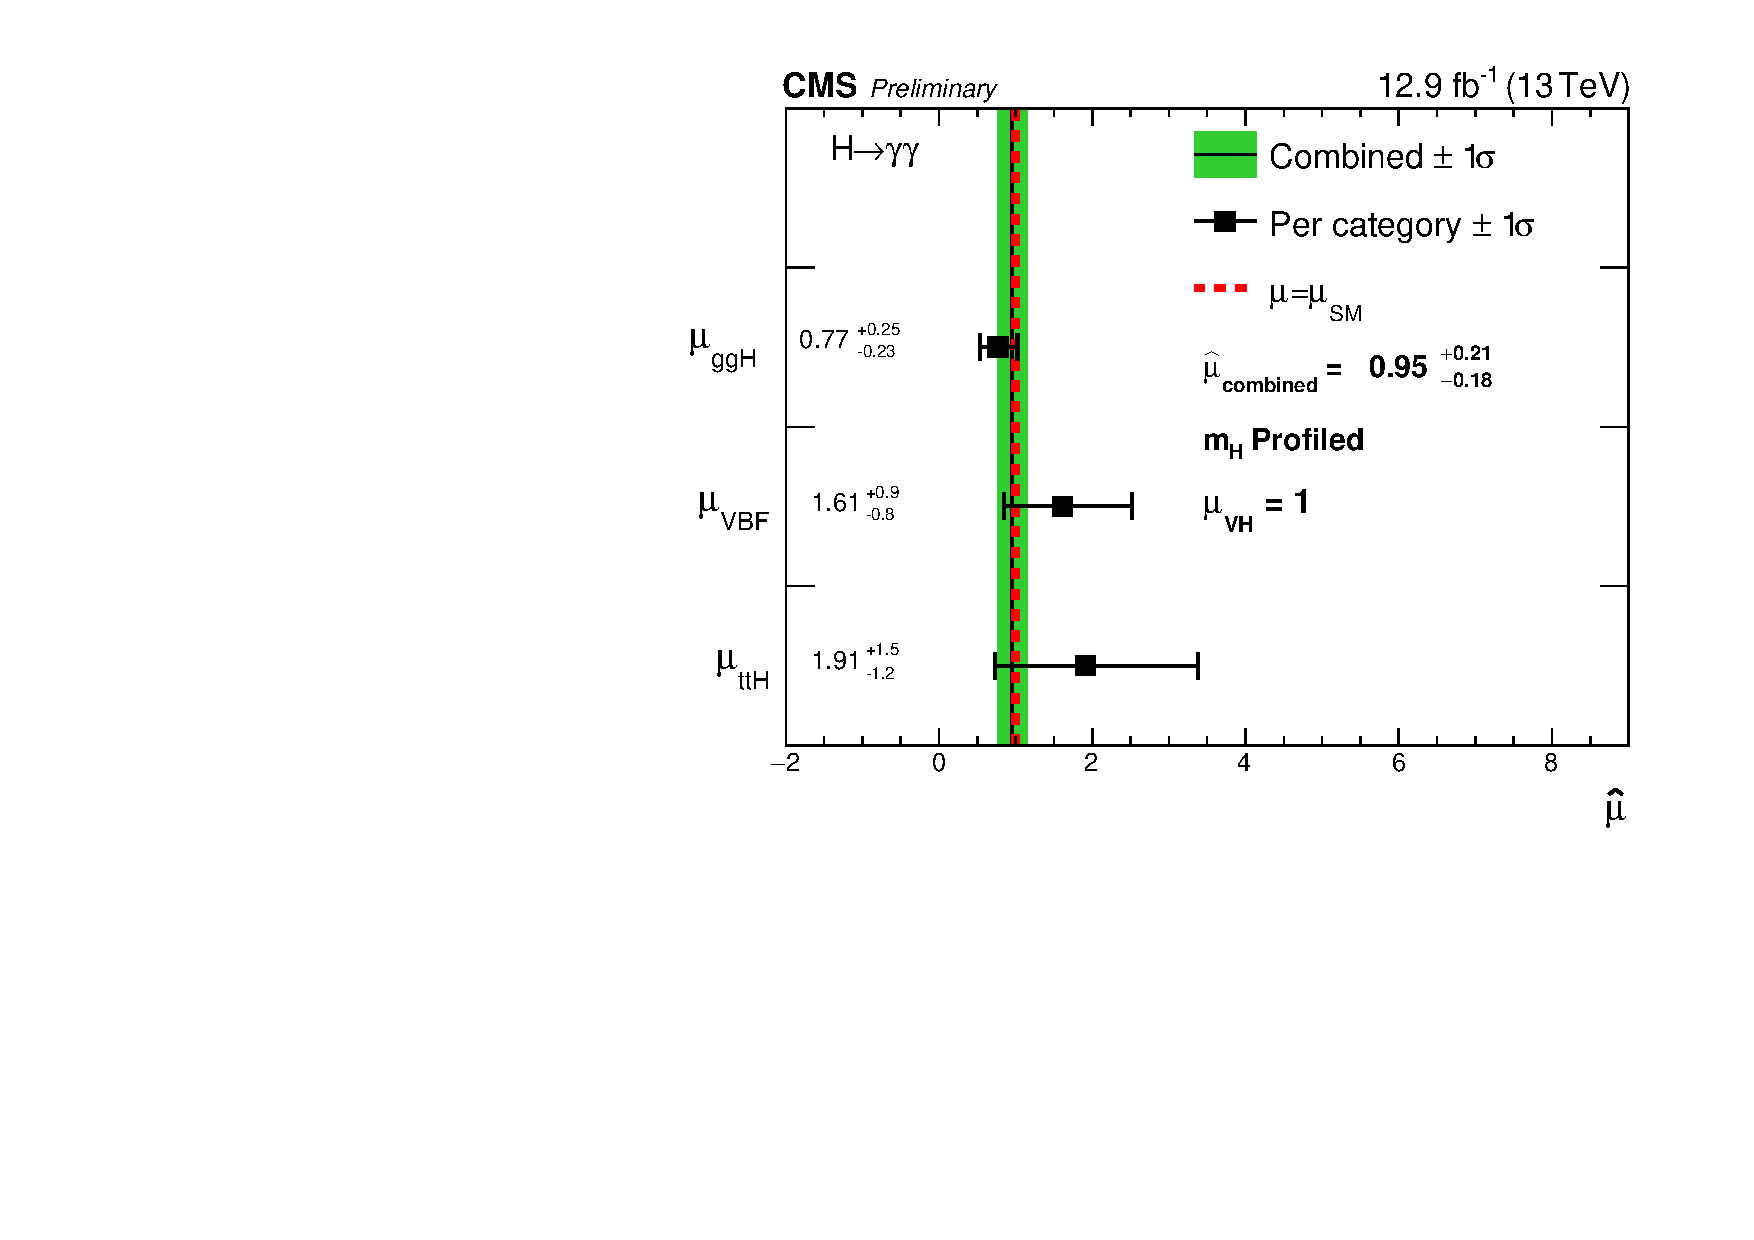
\includegraphics[width=1\textwidth]{statandresultsFigures/\whichFig/PerProcChannelCompatibilityProfileMH.pdf} 
\caption{The measurements of the per-process signal strengths \muggH, \muVBF, \muttH, obtained by performing \DNLL scans of each one while profiling the others. In each case \mH is also profiled in the fit, and $\muVH=1$ is imposed since this analysis does not include any categories specifically targeting the VH process. The vertical black line and green bands represent the measurement of the overall signal strength $\mu$, and the SM expectation is shown in the vertical red dashed line.}

\label{fig:statandresults:mu_per_proc}

\end{figure}

%\newpage
\subsection{Compatibility of result with SM in each category}

Using an analogous method to the one described in \Sec~\ref{sec:statandresults:mu_per_proc}, it is possible to make a measurement of the signal strength for each category separately. In this case, one \POI per analysis category is defined, which scales the yield of the signal models of all processes uniformly, but independently within each category. The full likelihood function is therefore expressed as:
\begin{equation}
\label{eq:statandresults:likelihood_function}
\mathcal{L}(\{\mu_C\}, \mH; \mathbf{n} | \mgg^{obs} ) = \prod_C \big[\mu_C \cdot f^C_S(\mgg^{obs,C} |\mH ; \mathbf{n}_S) + f^C_B(\mgg^{obs,C} | \mathbf{n}_B )\big], 
\end{equation}
where $\{\mu_C\}$ represents the set of signal strengths for each category.

Although the signal strengths $\{\mu_C\}$ do not have any direct physical meaning, they can be used to check that each category gives a result consistent with the overall measurement, and that no bias is introduced by any particular category. The result of the check is shown in \Fig~\ref{fig:statandresults:mu_per_tag}, which determines that all the per-category signal strengths are compatible with the \SM expectation and the overall result. The results for each per-category signal strength match those from~\cite{CMS-PAS-HIG-16-020} within a few a percent, as for previously quoted results. 

Of the eight categories which are included in this analysis, all but two of them (the \Untagged 2 and \VBFTag 0 categories ) fall within $1\sigma$ of the overall best-fit global signal strength, which roughly matches the expectation that a randomly distributed Gaussian variable falls within 1\sigma of the mean approximately 32\% of the time.

\begin{figure}[ht!]
\centering
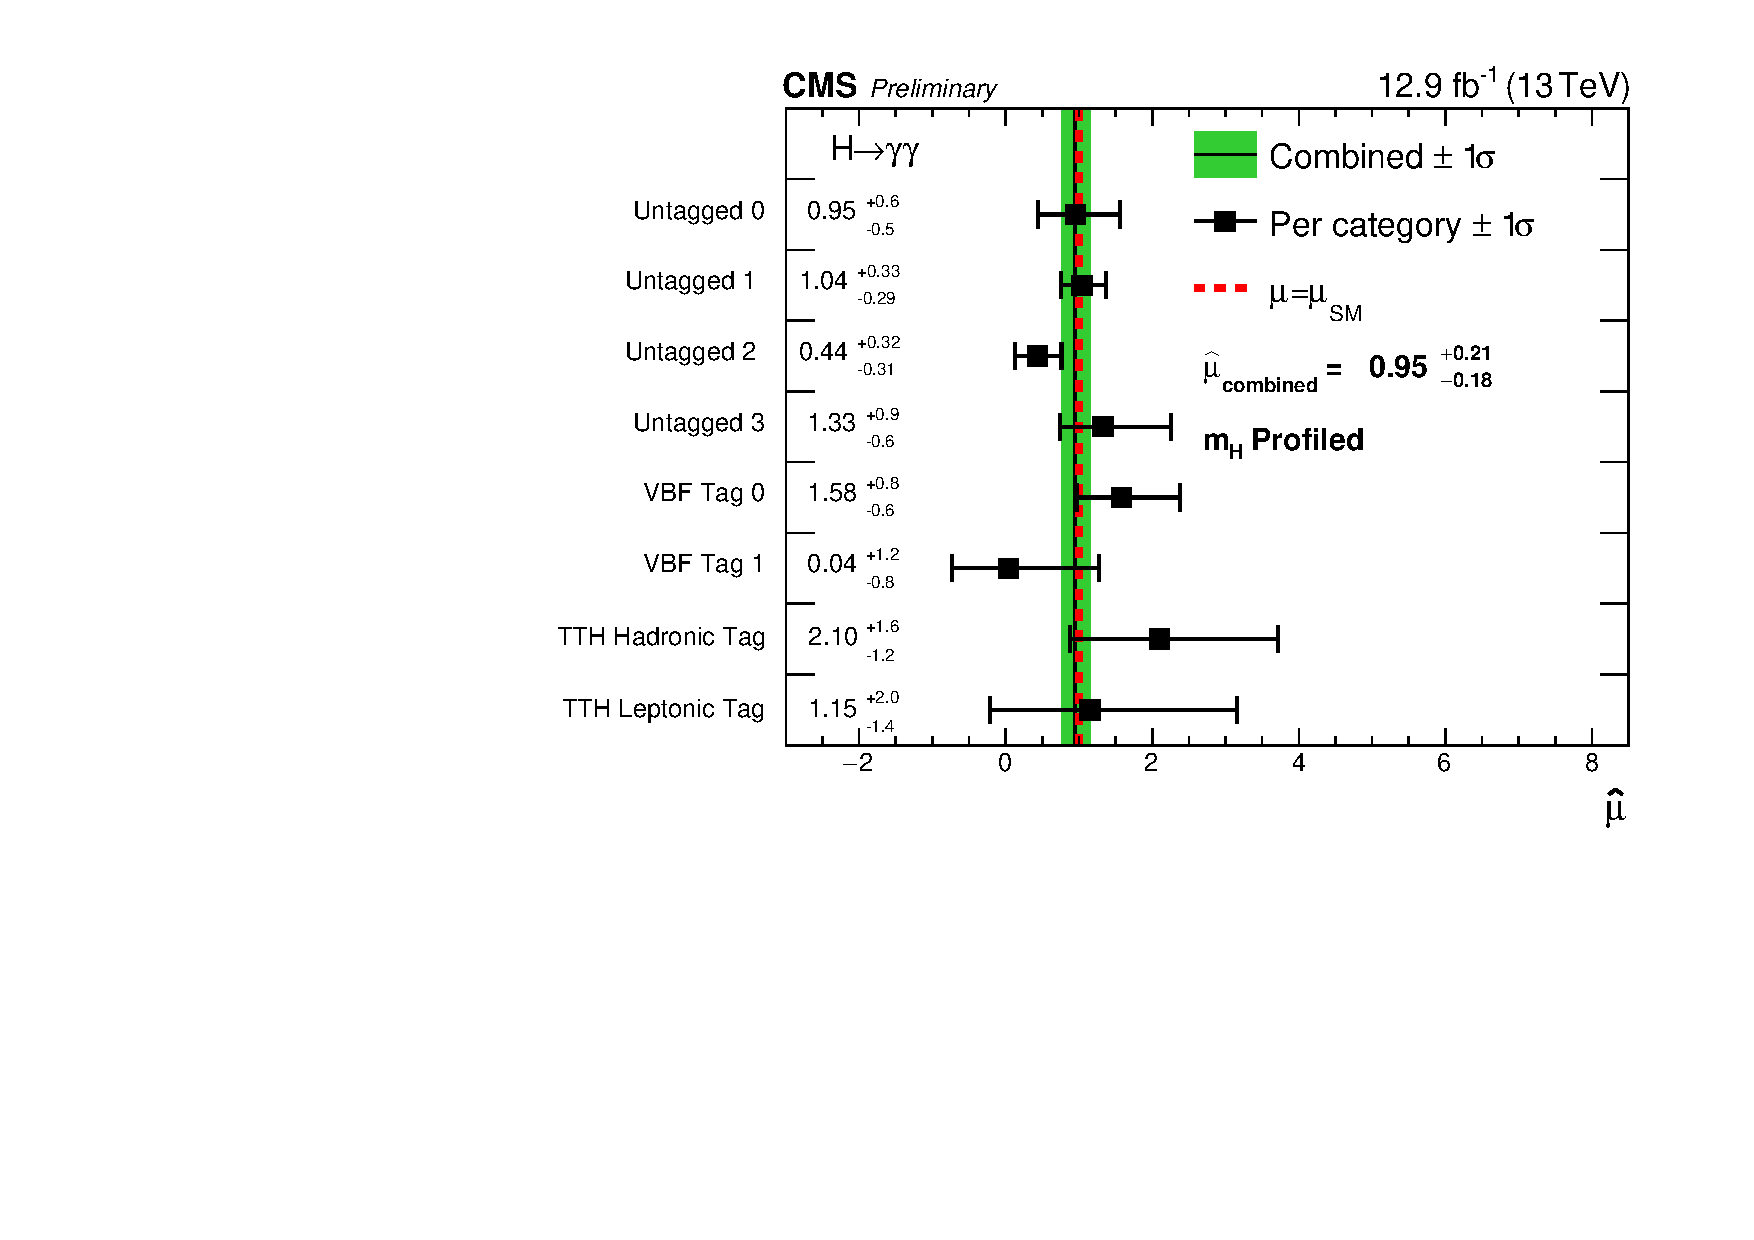
\includegraphics[width=1\textwidth]{statandresultsFigures/\whichFig/PerTagChannelCompatibilityProfileMH.pdf} 
\caption{The measurements of the per-category signal strengths, obtained by performing \DNLL scans of each one while profiling the others. In each case \mH is also profiled in the fit, The vertical black line and green bands represent the measurement of the overall signal strength $\mu$, and the SM expectation is shown in the vertical red dashed line. The per-category signal strengths do not have a direct physical interpretation, and this result is a check that no particular category is introducing a large bias into the overall measurement.}

\label{fig:statandresults:mu_per_tag}

\end{figure}

This result shows once again that the \Untagged categories are the ones which provide bulk of the sensitivity of the overall result. Another point of interest is that the $S/(S+B)$ of a given category does not necessarily correlate with the size of the uncertainty for that category. In particular, the category whose signal strength has the lowest uncertainty is the \Untagged 2 category, while \Fig~\ref{fig:model:sig_table_visualisation} shows that the \Untagged 0 category has the best $S/(S+B)$. This can be explained by the fact that the statistical component is still the dominating uncertainty in each measurement, and the lower $S/(S+B)$ of the \Untagged 2 category is compensated by the larger number of events which enter it. 

\section{Measurements of Higgs boson coupling modifiers}
\label{sec:statandresults:kappas}
\subsection{Motivation and theory}

The measurements presented so far have all dealt with Higgs boson signal strengths. Such observables are sensitive to variations in the rate at which the Higgs boson is produced, but do not take into account the possible variations in the partial width of the subsequent decay. An alternative set of measurements addresses this shortcoming by being sensitive to variations in the coupling strength of the Higgs boson with individual particles, relative to the \SM expectation. 

The so-called \emph{kappa} framework assigns a modifier to the coupling strength of the Higgs boson to a particle or group of particles $X$ directly in the amplitude of the process. The corresponding modifier is labelled as $\kappa_{X}$. A detailed description of the scheme is available in~\cite{Khachatryan:2016vau}. 
The assumptions which underly this framework are as follows: 
\begin{itemize}
\item any calculated deviations from the \SM prediction are due to only one Higgs-boson-like state with mass around 125\GeV;
\item the natural width of this state is sufficiently small that it can be neglected, allowing the \crosssection and branching fraction for a process $ii\rightarrow H \rightarrow ff$ to be decomposed as $(\sigma_{ii}^{H} \cdot \Gamma_{ff}^{H}) / (\Gamma_H)$, where $\sigma_{ii}^{H}$ is the \crosssection for a Higgs boson to be produced from the initial state $ii$, $\Gamma^{H}_{ff}$ is the partial decay width of the Higgs boson into the state $ff$ and $\Gamma_{H}$ is the total width of the Higgs boson.
\end{itemize}

The \emph{coupling modifier} $\kappa_{X}$ for a particle $X$ interacting with the Higgs boson is applied directly as a factor to the corresponding \crosssection $\sigma_{XX}^{H}$ or partial decay width $\Gamma^{H}_{XX}$. For processes which only occur via loops of particles, an \emph{effective coupling modifier} is defined as a function of the coupling modifiers for particles in which play a large role in the loop, e.g.~$\kappa_{\gamma} = \kappa_{\gamma}(\kappa_b, \kappa_t) $ (for the decay \Hgg) and $\kappa_{g} = \kappa_{g}(\kappa_b, \kappa_t) $ (for \ggH production).
Bosonic and fermionic coupling modifiers $\kf$ and $\kV$ are defined which uniformly scale the Higgs boson's interactions with all fermions and vector bosons respectively. The coupling modifiers applied to each of the main Higgs boson production processes and the \Hgg decay are shown in \Table~\ref{tab:statandresults:kappas}, adapted from~\cite{Khachatryan:2016vau}.

 \begin{table}[h]
 \resizebox{\textwidth}{!}{


 \begin{tabular} { |l | c | c | c | c | }
 \hline
 \hline
 Process & Type & Loop & Coupling modifier & Effective\\
 & & (interference)& (in terms of \kf and \kV)& coupling modifier\\
 \hline
 %\ggH & \crosssection & yes ($\Ptop$ - $\Pbottom$) & $1.06\cdot \kappa_t^2 + 0.01 \cdot \kappa_b^2 -0.07 \cdot \kappa_t\kappa_b (= \kf^2) $ & $\kappa_g^2$ \\
 \ggH & \crosssection & yes ($\Ptop$ - $\Pbottom$) & $\kf^2 $ & $\kappa_g^2$ \\
 \VBF & \crosssection & no & $ \kV^2$ & - \\
 \VH & \crosssection & no & $\kV^2$ & - \\
 \ttH & \crosssection & no & $\kf^2$ & - \\
 \hline
 \Hgg & partial width & yes ($\Ptop$ - $\PW$) & $1.59 \cdot \kV^2 + 0.07 \cdot \kf^2 - 0.66\cdot \kV \cdot \kf$ & $\kPho^2$ \\
 \hline
 \hline
 \end{tabular}

}
 \caption{Coupling strength modifiers attributed to each of the main Higgs boson production mechanism \crosssection\s and the partial width of the \Hgg decay, including QCD and EW corrections\quad\cite{Khachatryan:2016vau}.}
 \label{tab:statandresults:kappas}
\end{table}

\subsection{Bosonic and fermionic coupling modifiers}
To make a measurement of fermionic and bosonic Higgs boson coupling modifiers, the likelihood function is re-written such that \kf and \kV are the \POI\s: 
\begin{equation}
\label{eq:statandresults:likelihood_function_kvkf}
\begin{split}
\mathcal{L}(\kf,\kV, \mH; \mathbf{n} | \mgg^{obs} ) ={}&\prod_C \big[  f^C_B(\mgg^{obs,C} | \mathbf{n}_B )  \\ 
& + \kf^2\cdot(1.59\cdot\kV^2 + 0.07\kf^2 - 0.66\kV\kf) \cdot f^C_{S,{\text{ggH}}}(\mgg^{obs,C} |\mH ; \mathbf{n}_S) \\ 
& + \kf^2\cdot(1.59\cdot\kV^2 + 0.07\kf^2 - 0.66\kV\kf) \cdot f^C_{S,{\text{ttH}}}(\mgg^{obs,C} |\mH ; \mathbf{n}_S)  \\ 
& + \kV^2\cdot(1.59\cdot\kV^2 + 0.07\kf^2 - 0.66\kV\kf) \cdot f^C_{S,{\text{VBF}}}(\mgg^{obs,C} |\mH ; \mathbf{n}_S)  \\
& + \kV^2\cdot(1.59\cdot\kV^2 + 0.07\kf^2 - 0.66\kV\kf) \cdot f^C_{S,{\text{VH}}}(\mgg^{obs,C} |\mH ; \mathbf{n}_S)   \big]. 
\end{split}
\end{equation}
The definition of the test statistic is also modified to take the new \POI\s into account:
\begin{equation}
\label{eq:statandresults:test_statistic_kvkf}
 q(\kV,\kf)= -2 \ln \mathcal{L}(\kV,\kf,\hat{\mH}^{\mu}; \hat{\mathbf{n}}^{\mu}| \mgg^{obs})- 2\ln\mathcal{L}(\hat{\kV},\hat{\kf},\mH;\hat{\mathbf{n}}| \mgg^{obs} ).
\end{equation}
%where unlike \Eq~\ref{eq:statandresults:test_statistic_kvkf} there is no need to specify that the test statistic be null when the \POI\s are negative. The \mH parameter is profiled in this treatment.

The result of a two-dimensional \DNLL scan of \kf and \kV is shown in \Fig~\ref{fig:statandresults:kappa_plots_kvkf}. The black cross indicates the best-fit while the red diamond indicates the \SM expectation. The $1\sigma$ and $2\sigma$ contours are indicated by solid and dashed lines. The best-fit indicates compatibility with the \SM.The location of the best-fit point agrees within a few percent with the equivalent result in the \App of~\cite{CMS-PAS-HIG-16-020}. Measurements of \kf and \kV can be made individually following the same method as described in~\Sec{sec:statandresults:rvrf}. The \DNLL of each \POI while profiling the others can be found in \App~\ref{app:dnll_scans} in \Fig~\ref{fig:statandresults:kappa_per_v_and_f}, which yield the measurements:
\begin{equation*}
%\muFhat=0.82^{+0.27}_{-0.24} \text{ and } \muVhat=1.60^{+0.90}_{-0.76}.
\begin{split}
\obskV, \\
\obskF.
\end{split}
\end{equation*}

\begin{figure}[ht!]
\centering
\subfloat[\DNLL scan of \kf versus \kV]{
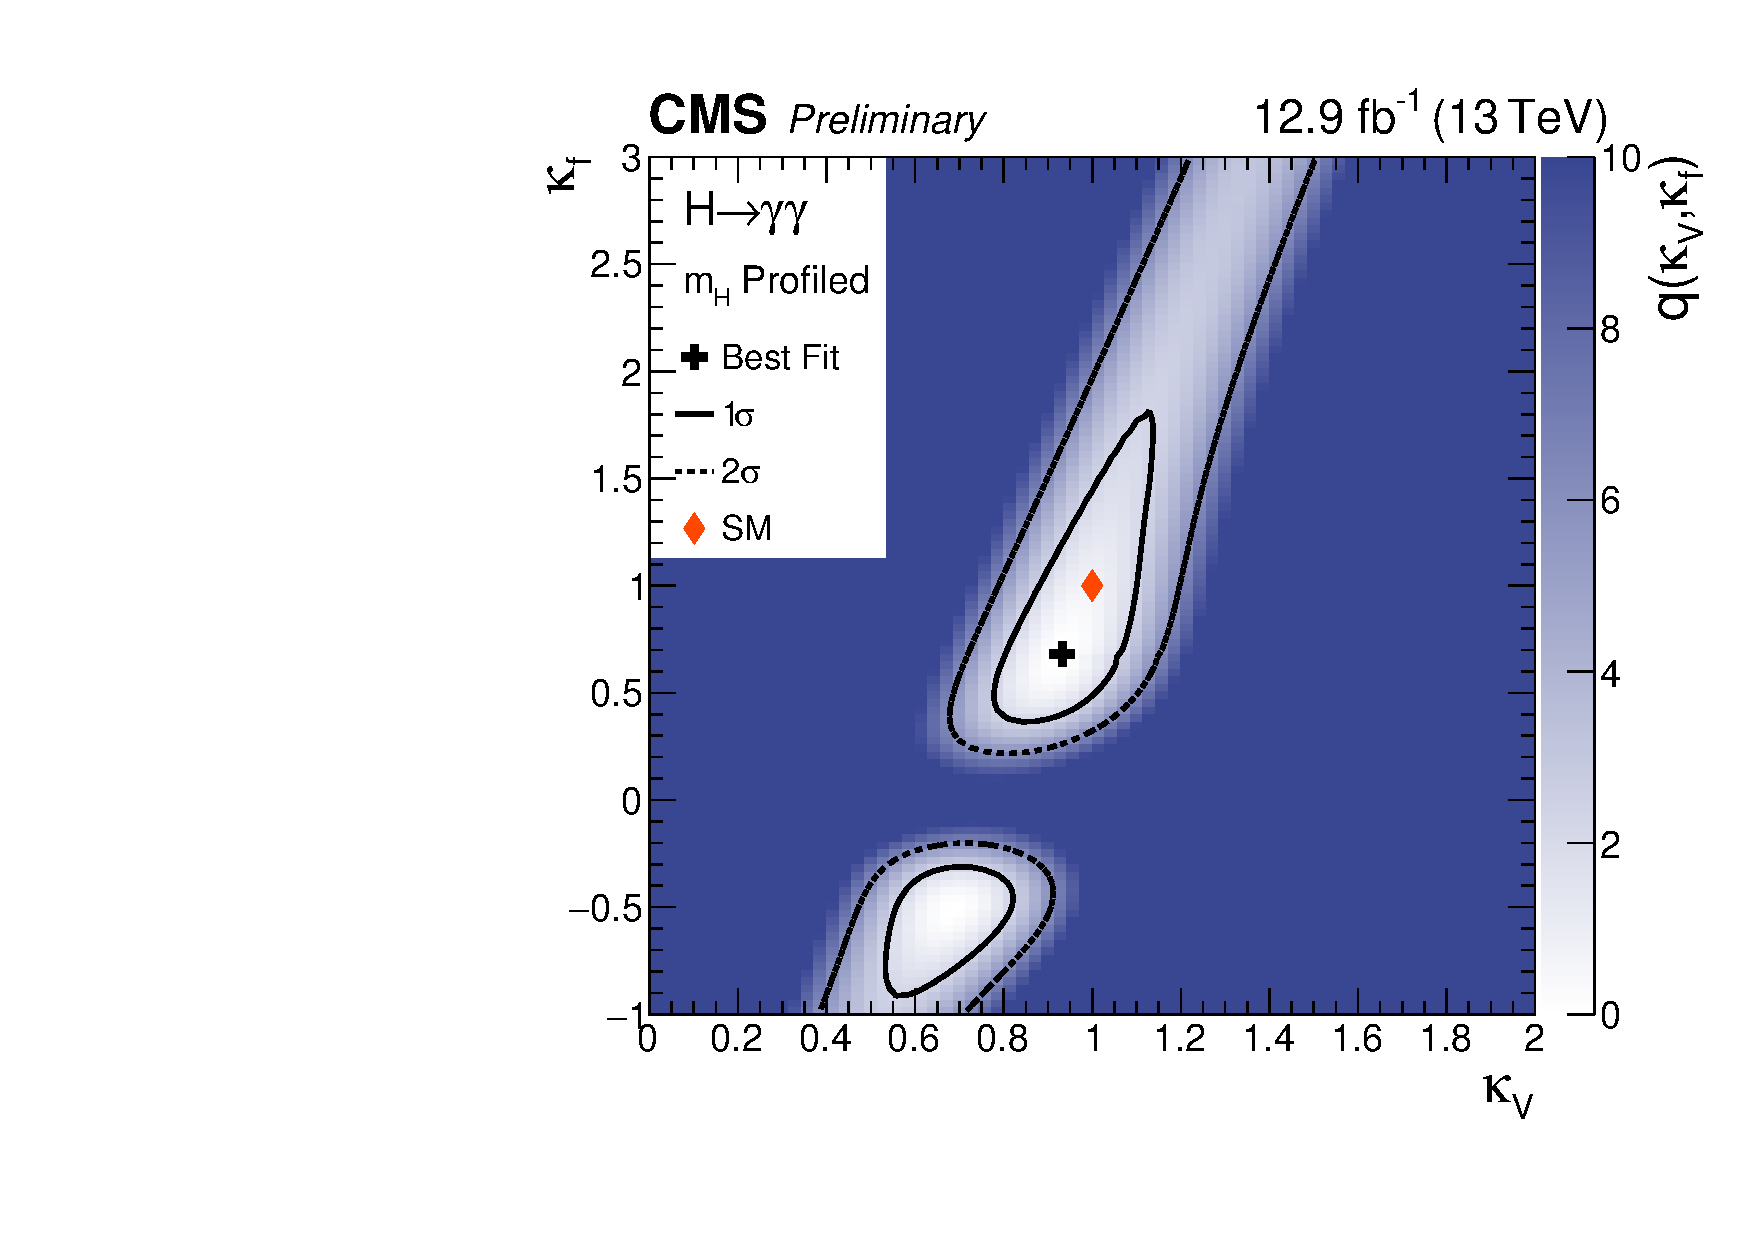
\includegraphics[width=0.75\textwidth]{statandresultsFigures/\whichFig/CVCFScanProfileMH_granular_col.pdf}}\\
%\subfloat[\DNLL scan of \kPho versus \kGlu]{
%\label{fig:statandresults:kappa_plots_kgkp}
%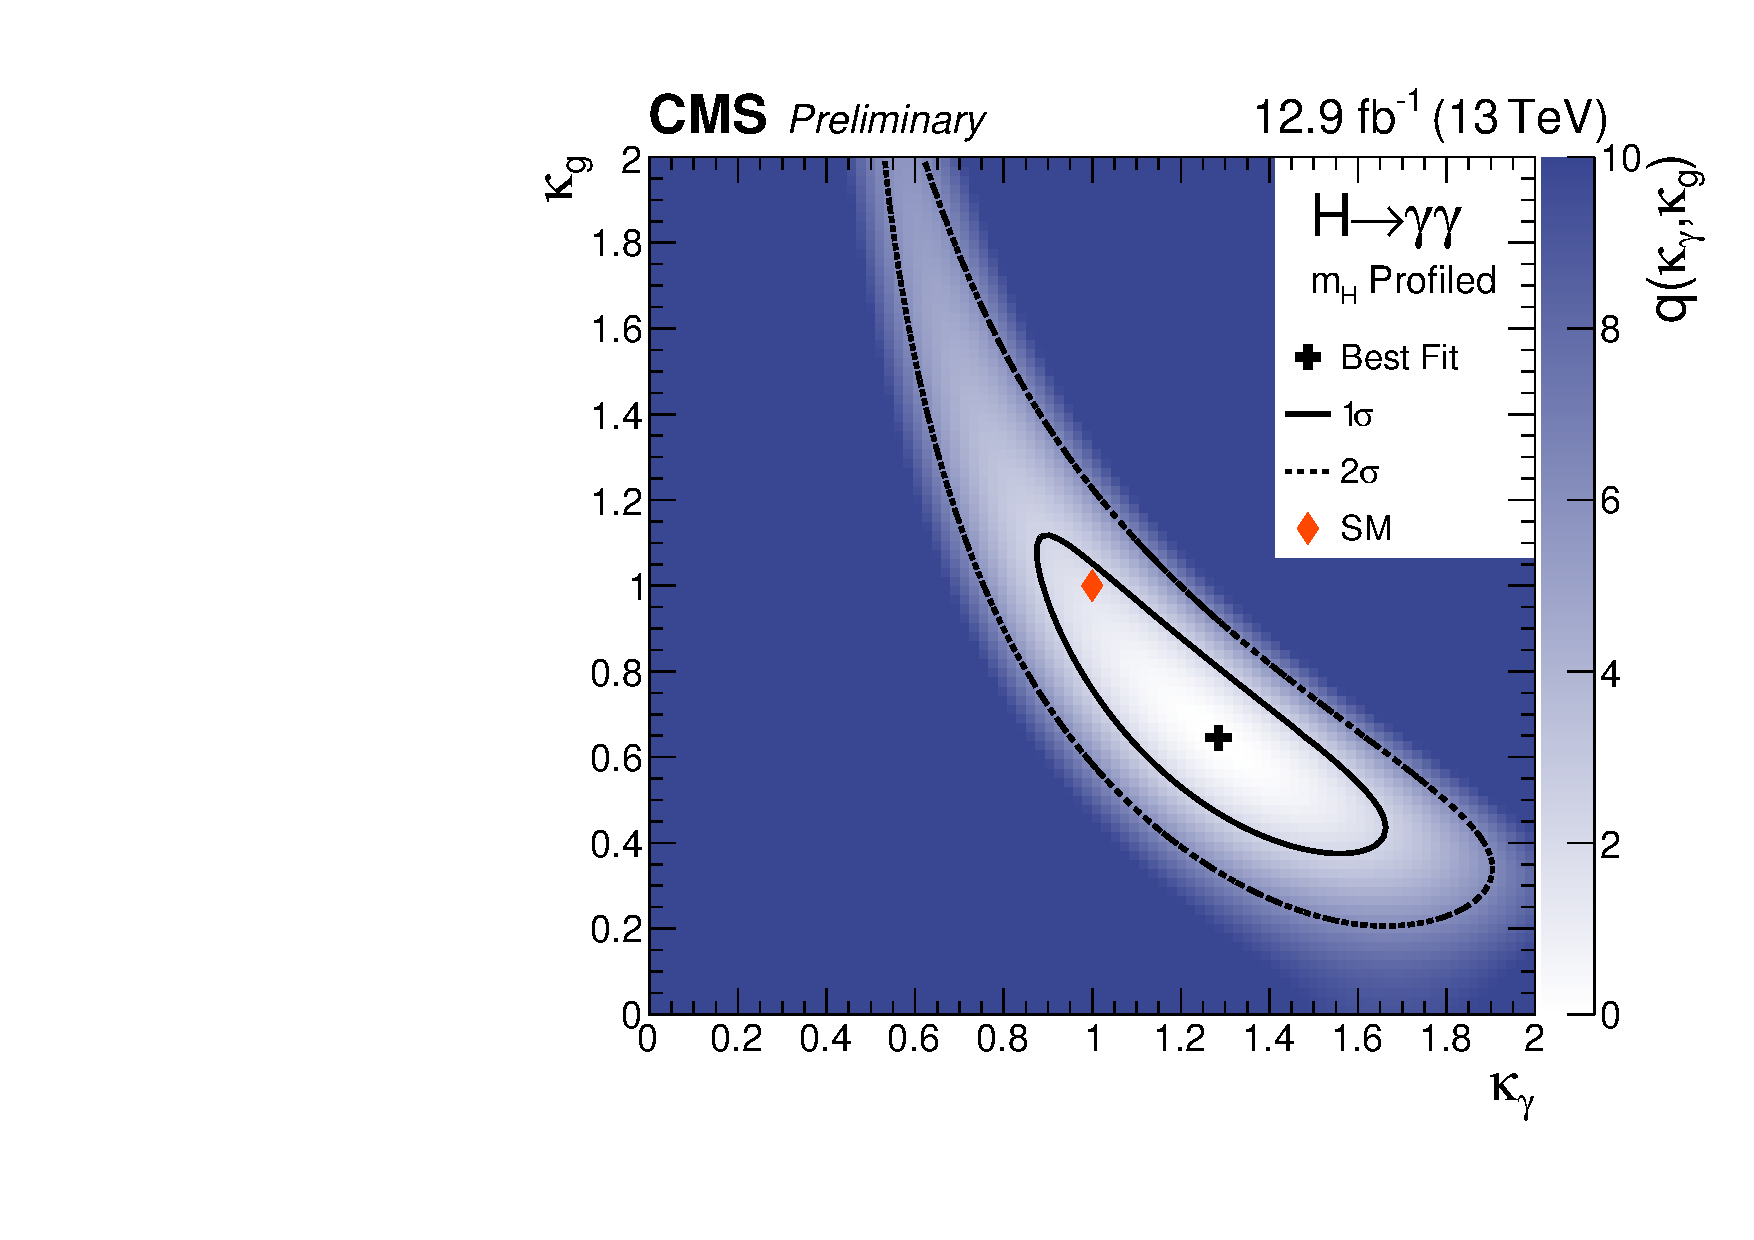
\includegraphics[width=0.65\textwidth]{statandresultsFigures/\whichFig/KGluKGamScanProfileMH_granular_col.pdf}}
%\caption{The result of a two-dimensional \DNLL scan of the effective coupling strength modifiers for: fermions and bosons (a), and gluons and photons (b). The best-fit values are denoted with black crosses and the SM expected values with red diamonds. The best-fit points agree with the SM within the $1\sigma$ and $2\sigma$ uncertainty contours denoted by the solid and dashed lines respectively.}
\caption{The result of a two-dimensional \DNLL scan of the effective coupling strength modifiers for fermions and bosons (a). The best-fit values are denoted with black crosses and the SM expected values with red diamonds. The best-fit points agree with the SM within the $1\sigma$ and $2\sigma$ uncertainty contours denoted by the solid and dashed lines respectively.}
%\label{fig:statandresults:kappa_plots}
\label{fig:statandresults:kappa_plots_kvkf}
\end{figure}

An interesting feature of \Fig~\ref{fig:statandresults:kappa_plots_kvkf} is that a second local minimum exists where \kf takes negative values. In general, the coupling strength modifiers always occur squared in the amplitude. However, as noted in \Table~\ref{tab:statandresults:kappas}, the \Hgg amplitude contains destructive interference between the contributions of the $\Ptop$ and $\PW$ result in a term proportional to $(\kV\cdot\kf)$. This means that the measurement has a small amount of sensitivity to the sign of the coupling strength modifier $\kf$. In this measurement, the positive value is preferred, as expected by the \SM.


%\begin{figure}[ht!]
%\centering
%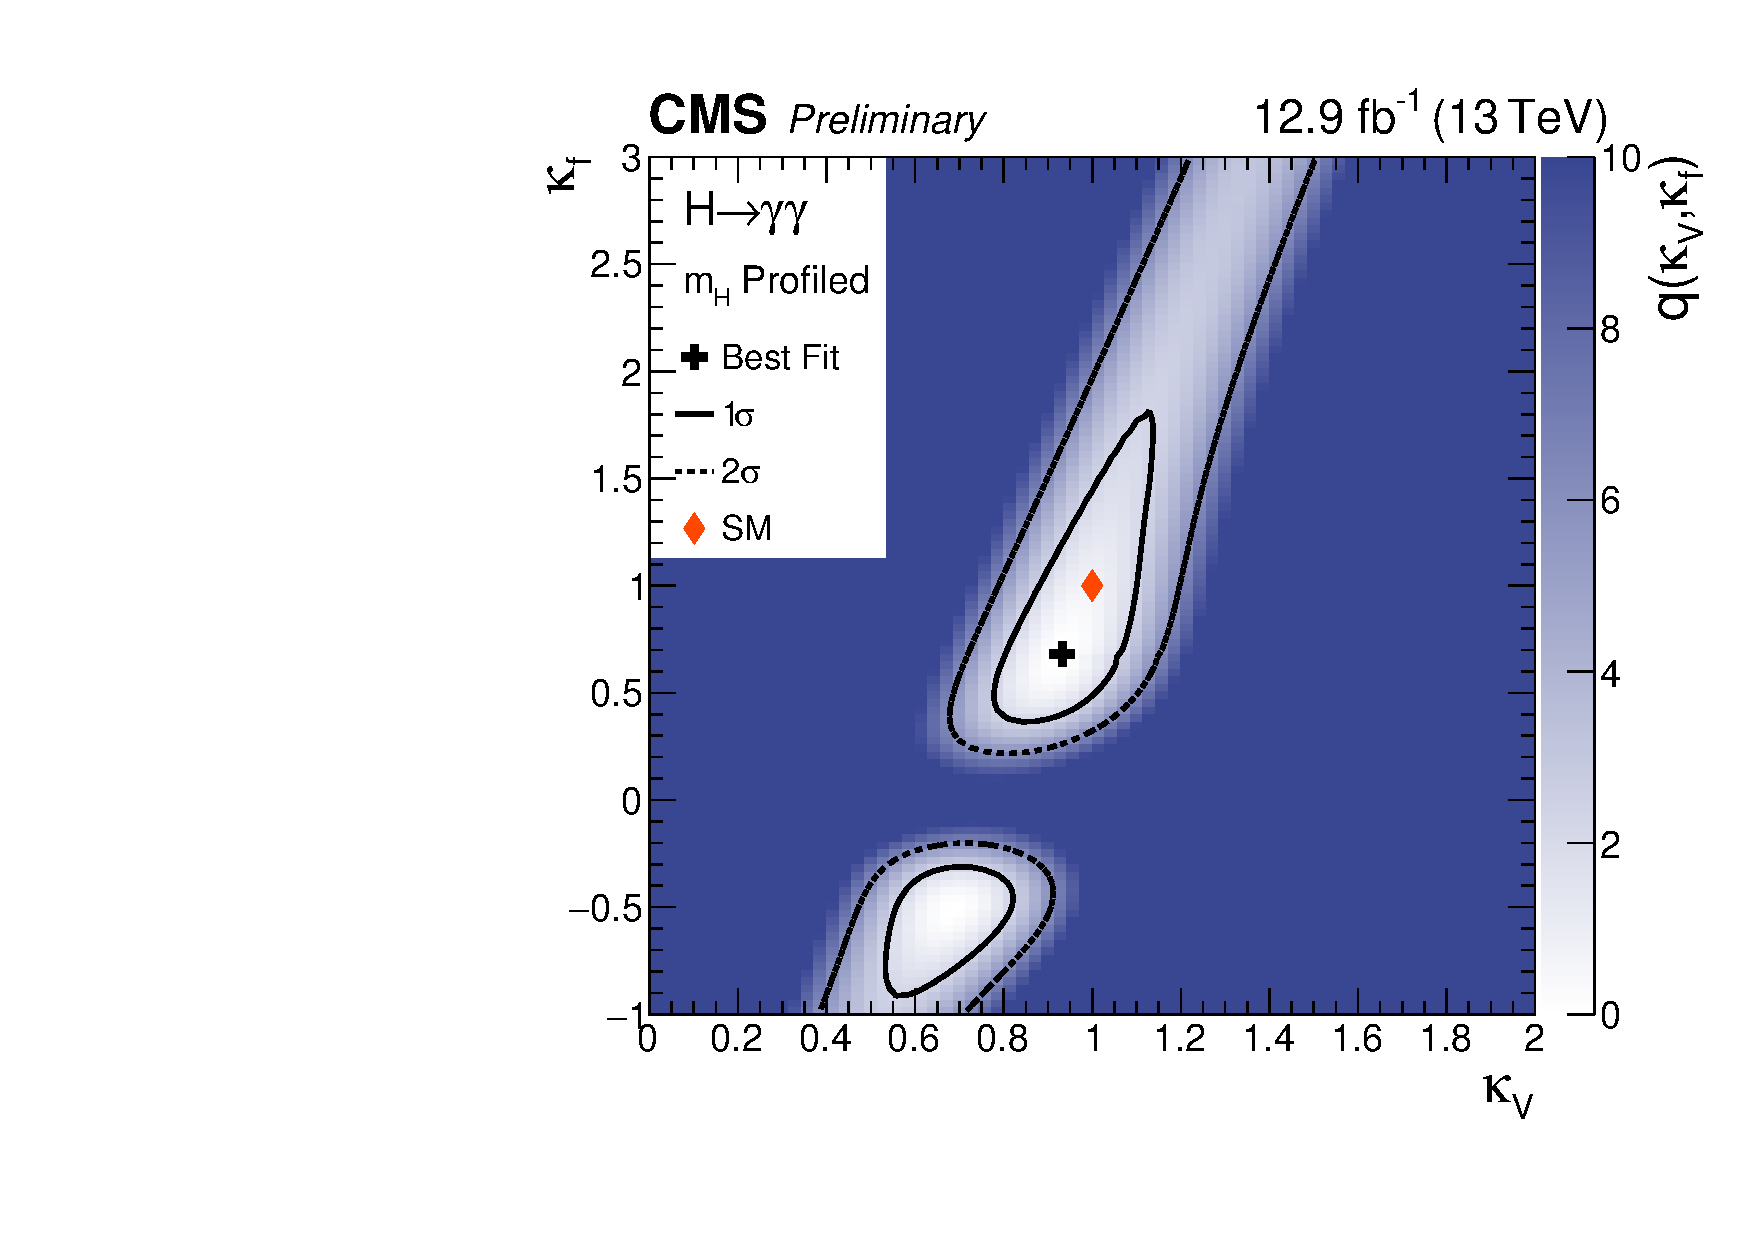
\includegraphics[width=0.6\textwidth]{statandresultsFigures/\whichFig/CVCFScanProfileMH_granular_col.pdf} 
%\caption{The result of a two-dimensional \DNLL scan of the coupling strength modified for fermions (\kf ) and vector bosons (\kV ). The best fit value is denoted with a black cross and the SM expected value with a red diamond. The best-fit agrees with the SM within the $1\sigma$ and $2\sigma$ uncertainty contours denoted by the solid and dashed lines respectively.}
%
%\label{fig:statandresults:kappa_plots_kvkf}
%\end{figure}

\subsection{Effective coupling modifiers to gluons and photons}
Alternatively, the measurement can be made in terms of the Higgs boson's effective coupling to gluons and photons using a two-dimensional \DNLL scan of \kGlu and \kPho. In this case, the likelihood function is modified as follows:
\begin{equation}
\label{eq:statandresults:likelihood_function_kgkg}
\begin{split}
 \mathcal{L}(\kf,\kV, \mH; \mathbf{n} | \mgg^{obs} ) = \prod_C \big[{}&f^C_B(\mgg^{obs,C} | \mathbf{n}_B ) \\ 
&+ \kGlu^2\cdot \kPho^2 \cdot f^C_{S,{\text{ggH}}}(\mgg^{obs,C} |\mH ; \mathbf{n}_S) \\ 
&+ \kPho^2\cdot f^C_{S,{\text{ttH}}}(\mgg^{obs,C} |\mH ; \mathbf{n}_S) \\ 
&+ \kPho^2\cdot f^C_{S,{\text{VBF}}}(\mgg^{obs,C} |\mH ; \mathbf{n}_S) \\
&+ \kPho^2\cdot f^C_{S,{\text{VH}}}(\mgg^{obs,C} |\mH ; \mathbf{n}_S)\quad\big].
\end{split}
\end{equation}
The test statistic $q(\kPho,\kGlu)$ is then defined analogously to \Eq~\ref{eq:statandresults:test_statistic_kvkf}.
In this case the \mH parameter is profiled. The results of the \DNLL scan are presented in \Fig~\ref{fig:statandresults:kappa_plots_kgkp}.

\begin{figure}[ht!]
\centering
%\subfloat[\DNLL scan of \kf versus \kV]{
%\label{fig:statandresults:kappa_plots_kvkf}
%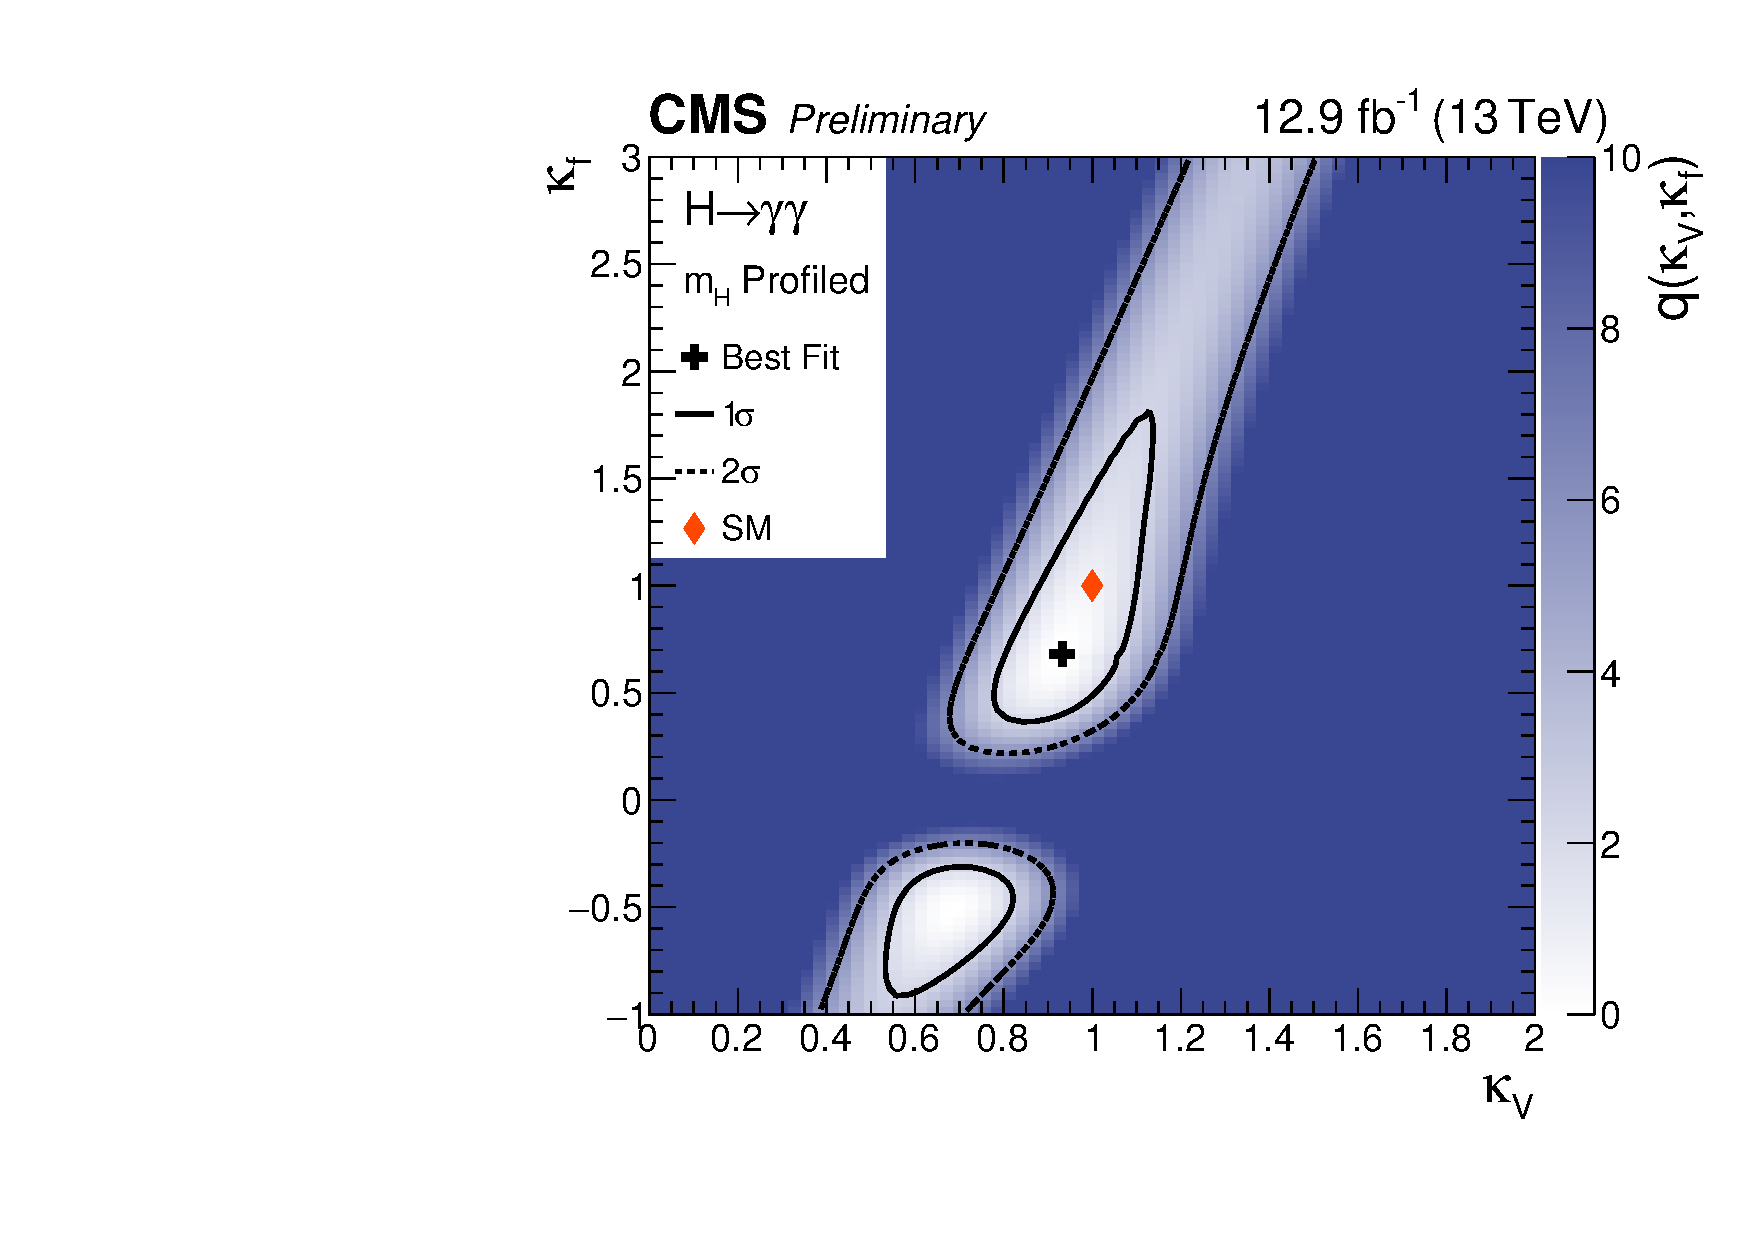
\includegraphics[width=0.65\textwidth]{statandresultsFigures/\whichFig/CVCFScanProfileMH_granular_col.pdf}}\\
\subfloat[\DNLL scan of \kPho versus \kGlu]{
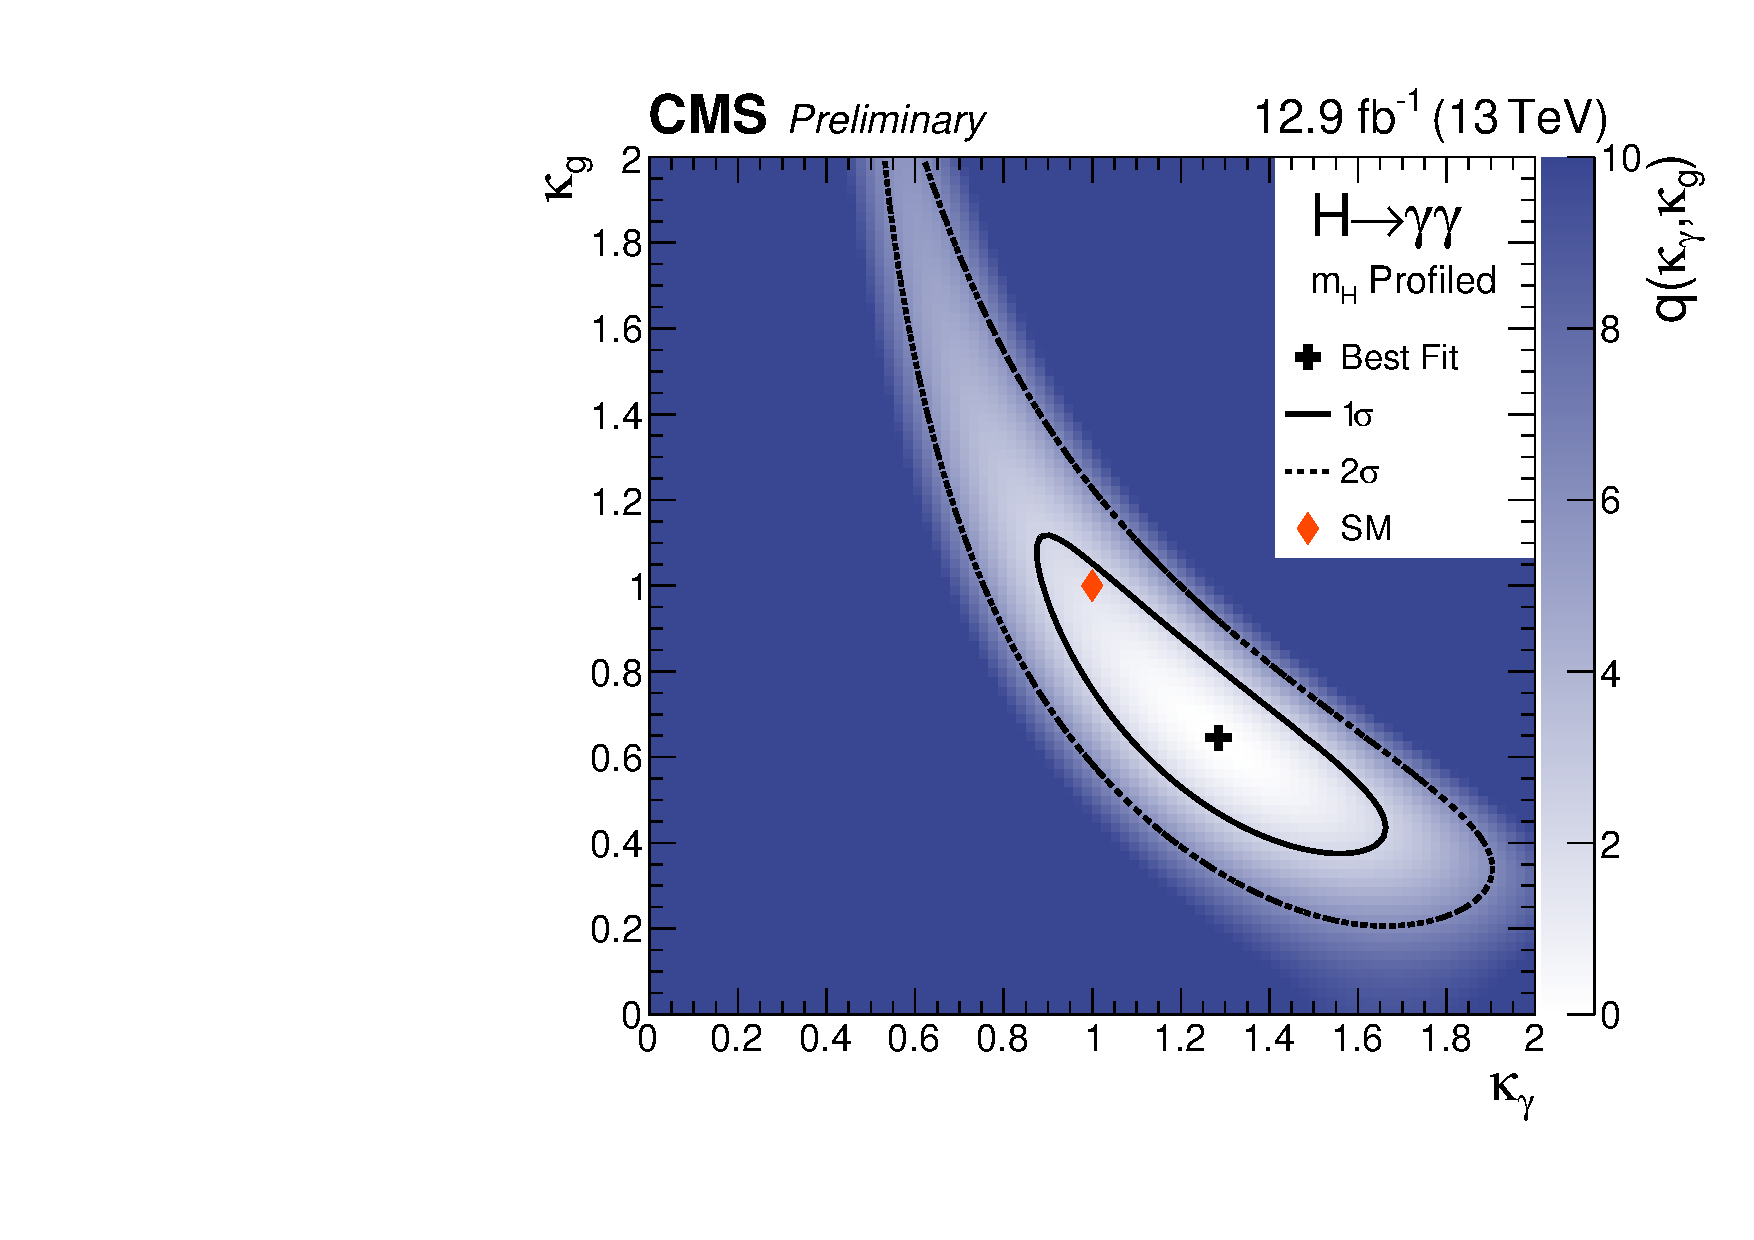
\includegraphics[width=0.75\textwidth]{statandresultsFigures/\whichFig/KGluKGamScanProfileMH_granular_col.pdf}}
\caption{The result of a two-dimensional \DNLL scan of the effective coupling strength modifiers for gluons and photons. The best-fit values are denoted with black crosses and the SM expected values with red diamonds. The best-fit points agree with the SM within the $1\sigma$ and $2\sigma$ uncertainty contours denoted by the solid and dashed lines respectively.}
\label{fig:statandresults:kappa_plots_kgkp}
%\label{fig:statandresults:kappa_plots}
\end{figure}
Measurements of \kGlu and \kPho are performed by producing a \DNLL of each \POI while profiling the other.
The scans are available in \App~\ref{app:dnll_scans} in \Fig~\ref{fig:statandresults:kappa_per_g_and_g}, which yield the measurements:
\begin{equation*}
%\muFhat=0.82^{+0.27}_{-0.24} \text{ and } \muVhat=1.60^{+0.90}_{-0.76}.
\begin{split}
\obskGlu, \\
\obskPho.
\end{split}
\end{equation*}

The best-fit point agrees with the \SM within the uncertainties. In this case, there is no sensitivity to negative values of the modifiers, since the \Hgg loop which contains a term proportional to $(\kV\cdot\kf)$ is contained in the effective coupling \kPho. 



